\documentclass[11pt,twoside,a4paper]{article}
\usepackage[hmargin=2cm, vmargin=2cm]{geometry}
\usepackage{microtype}
\usepackage{graphicx}
\usepackage[english]{babel}
\usepackage{setspace}
\usepackage{xcolor}
\usepackage{multicol}
\usepackage{multirow}
\usepackage{float}
\usepackage{subcaption} 
\usepackage{amsmath}
\usepackage{amsthm}
\usepackage{amssymb}
\usepackage[hidelinks=true]{hyperref}
\usepackage{overpic}
\usepackage[font=small,skip=2pt]{caption}

\newcommand{\independent}{\perp\!\!\!\!\perp} 

\onehalfspacing
\parindent=0pt
\usepackage{pagecolor}
\pagecolor{white}

\begin{document}

\begin{titlepage}
  \centering
  {\LARGE\bfseries Dimension Reduction in Regression: \\ Comparative Analysis of Principal Component Regression and Partial Least Squares\par}
  \vfill
  {\Large Khabibullo Ibadullaev, Bekhzod Abulov\par}
  \vfill
  {\large \today\par}
  \vfill
  {\large University of Bonn\par}
  {\large Research Module in Econometrics and Statistics\par}
  {\large Supervised by: Prof. Dr. Joachim Freyberger\par}
  \vfill
  {\large Winter Semester 2024/2025\par}
\end{titlepage}

\newpage

\thispagestyle{empty}
\tableofcontents

\newpage

\setlength{\abovedisplayskip}{0.35cm}
\setlength{\belowdisplayskip}{0.35cm}

\setlength{\abovedisplayshortskip}{0.2cm}
\setlength{\belowdisplayshortskip}{0.35cm}
\setlength{\parskip}{0.5em}
\pagenumbering{arabic}

\section{Introduction}

Regression models are a fundamental tool in statistical modeling, enabling the prediction of a dependent variable based on a set of independent variables. However, in modern applications, datasets often exhibit high-dimensionality, where the number of predictors (\( p \)) is significantly larger than the number of observations (\( n \)). This scenario, commonly referred to as the curse of dimensionality, poses significant challenges to traditional regression methods, particularly Ordinary Least Squares (OLS) regression.

One of the primary concerns in high-dimensional regression is multicollinearity—a situation where predictor variables are highly correlated. Multicollinearity leads to inflated standard errors, unstable coefficient estimates, and difficulties in interpreting model parameters. Additionally, high-dimensional models tend to overfit the training data, resulting in poor generalization to unseen observations. Computational complexity further exacerbates these challenges, making it difficult to estimate model parameters efficiently.

To address these issues, researchers have developed dimension reduction techniques that aim to transform high-dimensional predictor spaces into lower-dimensional representations while preserving essential information. Two widely used techniques in this context are Principal Component Regression (PCR) and Partial Least Squares (PLS). These methods construct new predictor variables, referred to as components, that capture the most relevant variation in the dataset.
The use of PCR and PLS is prevalent in various disciplines, including chemometrics, finance, genomics, and environmental science, where datasets often contain a large number of correlated predictors. While both methods offer solutions to the high-dimensional regression problem, they differ in their approach, underlying assumptions, and effectiveness in different scenarios.

This paper provides a comprehensive analysis of  Principal Component Regression (PCR) and Partial Least Squares (PLS), focusing on their theoretical foundations, practical implementations, and empirical performance evaluation across various regression settings. Specifically, in Section 2 we investigate the mathematical principles underlying these methods, highlighting their similarities and differences in handling multicollinearity and dimensionality reduction. A key focus in Section 3 is on understanding the bias-variance trade-off by performing a detailed Mean Squared Error (MSE) decomposition of regression coefficients, as well as evaluating predictive performance through Cross-Validation (CV) MSE. The study systematically compares these methods in different scenarios. To further assess model stability and generalization ability, a Monte Carlo simulation is conducted using synthetic datasets, allowing for an in-depth examination of performance under varying levels of correlation. Additionally, in Section 4 both PCR and PLS are applied to real-world regression problems, including Near-Infrared (NIR) Spectroscopy for Moisture Prediction, to evaluate their practical utility and interpretability. Finally, in Section 5 we discuss the strengths and weaknesses of each method, providing guidance on when to prefer PCR over PLS (or vice versa) and exploring potential hybrid approaches that integrate the advantages of both techniques.
\newpage

\section{Theory}

Traditional regression methods, such as OLS, assume that the predictor matrix \( X \) has full rank, ensuring a unique solution for the estimated coefficients. However, in many practical applications, datasets exhibit high collinearity among predictors or even contain more predictors than observations (\( p \gg n \)), making \( X^T X \) nearly singular or non-invertible. This leads to large variances in coefficient estimates, making the regression model highly unstable. The instability of OLS is evident in the variance expression:
\begin{equation} 
\text{Var}(\hat{\beta}_{\text{OLS}}) = \sigma^2 (X^T X)^{-1}
\end{equation}
Applying the eigen-decomposition:
\begin{equation}
X^T X = Q \Lambda Q^T
\end{equation}
we obtain:
\begin{equation}
\text{Var}(\hat{\beta}_{\text{OLS}}) = \sigma^2 Q \Lambda^{-1} Q^T
\end{equation}
where \( \Lambda \) contains the eigenvalues of \( X^T X \), we observe that when multicollinearity is present, some eigenvalues approach zero, making \( \Lambda^{-1} \) contain large values, which significantly inflates the variance of \( \hat{\beta}_{\text{OLS}} \).

PCR and PLS overcome this issue by constructing a set of orthogonal predictors, thereby improving numerical stability and reducing overfitting. While,  PCR mitigates this issue by removing components corresponding to small eigenvalues, ensuring that the variance of the estimated coefficients remains controlled, PLS focuses on components that maximize the covariance with \( Y \), eliminating high-variance directions that contribute to unstable coefficient estimates, ensuring a more robust regression model.


\subsection{Principal Component Regression (PCR)}

Principal Component Regression (PCR) is a widely used statistical technique that integrates Principal Component Analysis (PCA) with Ordinary Least Squares (OLS) regression to address issues of high-dimensionality and multicollinearity in regression problems. The fundamental idea behind PCR is to transform the original predictor variables, which may be highly correlated, into a new set of uncorrelated variables called principal components (Figure 1). Regression is then performed using a selected subset of these principal components, effectively reducing the dimensionality of the predictor space while mitigating instability in coefficient estimates.

PCR is an effective tool for dealing with multicollinearity, it is important to note that it is an unsupervised method, meaning that the principal components are chosen solely based on variance in the predictor space, without considering the response variable \( Y \). This characteristic distinguishes it from methods like Partial Least Squares (PLS), which optimize component selection based on predictive relevance to \( Y \).

\newpage
\paragraph{Mathematical Formulation} \ \

The key steps of PCR are as follows:

\begin{enumerate}
    \item Perform \textbf{Principal Component Analysis (PCA)} on \( X \), which involves computing the \textbf{Singular Value Decomposition (SVD)}:
   \begin{equation}
    X = U \Sigma V^T
    \end{equation}
    where:
    \begin{itemize}
        \item \( U \) is an \( n \times n \) orthogonal matrix (left singular vectors),
        \item \( \Sigma \) is an \( n \times p \) diagonal matrix with singular values,
        \item \( V \) is a \( p \times p \) orthogonal matrix (right singular vectors), whose columns are the principal component directions.
    \end{itemize}
    
    \item Transform the original predictors into principal components:
    \begin{equation}
    Z = X V
    \end{equation}
    where  \( Z \) represents the uncorrelated principal components of X.
 
    \item Perform OLS regression on the transformed dataset:
    \begin{equation}
    Y = Z \gamma + \epsilon
    \end{equation}
    where \( \gamma \) is the transformed coefficient vector in the principal component space.
  \end{enumerate}
  
 \paragraph{Unsupervised Nature of PCR} \ \

PCR is fundamentally an \textbf{unsupervised} technique because it selects principal components based on variance in \( X \) without considering \( Y \). This is evident from the PCA decomposition:
\begin{equation}
X^T X = V \Lambda V^T
\end{equation}
Since \( V \) is computed purely from \( X \), it does not incorporate \( Y \). As a result, PCR may discard components that contain important predictive information for \( Y \), making it less efficient for regression tasks compared to supervised alternatives like PLS.

\begin{figure}[H]
    \centering
    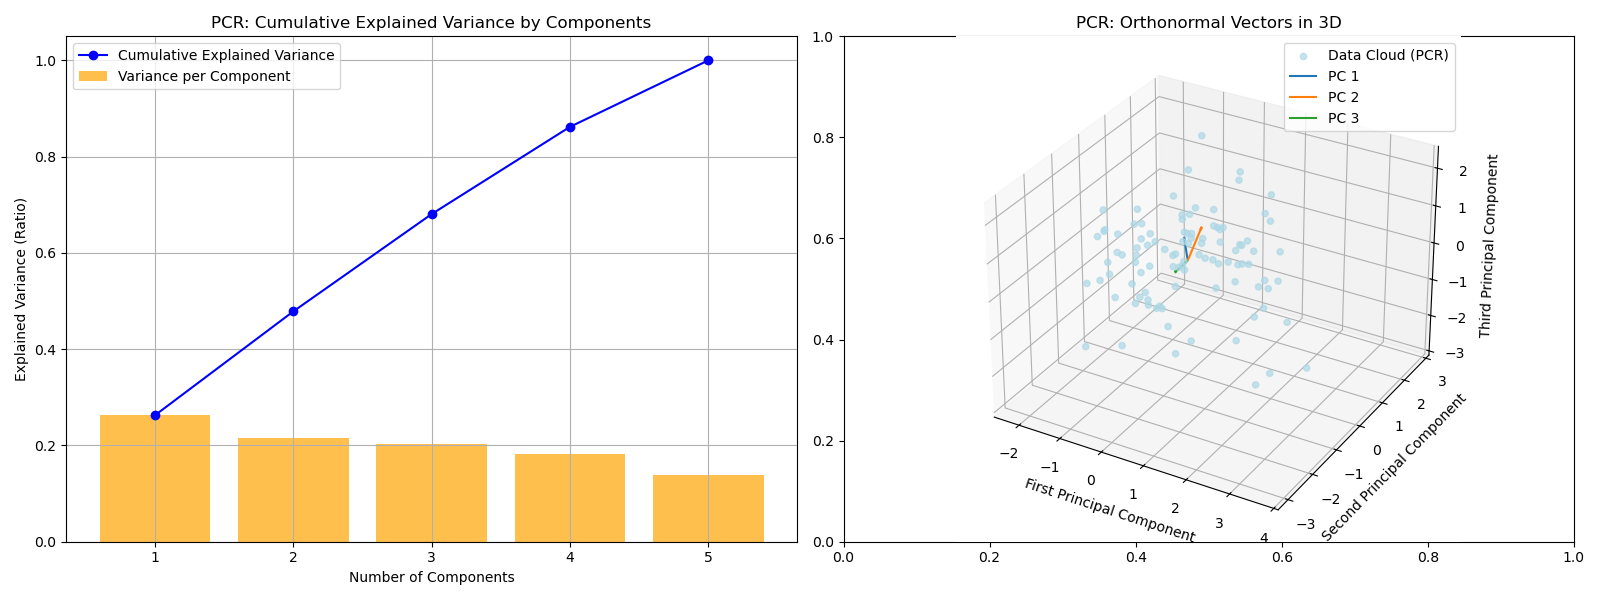
\includegraphics[width=0.9\textwidth]{PCR_Selected_Analysis.png}
    \caption{Principal Component Regression (PCR) Analysis Results}
    \label{fig:PCR_analysis}
\end{figure}

\newpage
\paragraph{Variance Reduction and Bias in PCR}  \ \

A key feature of PCR is its ability to reduce variance in estimated coefficients by using only first \( k \) principal components and eliminating components associated with small eigenvalues:
   \begin{equation}
    Z_k = X V_k
    \end{equation}
    
Estimating regression coefficients in the principal component space:    
    \begin{equation}
\hat{\gamma_k} = (Z_k^T Z_k)^{-1} Z_k^T Y
\end{equation}

Using the eigen decomposition (7), we obtain:
\begin{equation}
\hat{\gamma_k}  = \Lambda_k^{-1} V_k^T X^T Y
\end{equation}
    where \( \Lambda_k \) contains only the top \( k \) eigenvalues of \( X^T X \), while \( V_k \) consists of the first \( k \) principal components that capture the most variance in \( X \). The selection of \( k \) is often done using cross-validation or based on the cumulative explained variance criterion (Figure 1).

Transforming back to the original space:
\begin{equation}
\hat{\beta}_{\text{PCR}} = V_k \hat{\gamma_k} = V_k \Lambda_k^{-1} V_k^T X^T Y
\end{equation}
Recall that OLS can be written in terms of PCA decomposition (7). If all principal components are used (\( k \) = \( p \)), then we have:
\begin{equation}
\hat{\beta}_{\text{PCR}} = \hat{\beta}_{\text{OLS}} = V \Lambda^{-1} V^T X^T Y
\end{equation}

Which confirms that, by discarding small eigenvalues, PCR inherently reduces variance, albeit at the cost of introducing some bias. This trade-off is similar to ridge regression and is crucial in high-dimensional settings. Even though we are selecting a subset of principal components, Eckart-Young theorem guarantees that using the first \( k \) principal components in PCR is the best way to approximate and reduce dimensionality while preserving the most important information.

Principal Component Regression provides a robust approach for handling multicollinearity and high-dimensional data. However, its unsupervised nature may lead to suboptimal predictive performance, as it does not consider the response variable in component selection. In the next section, we introduce Partial Least Squares (PLS), which addresses this limitation by incorporating response information into the component selection process.

\subsection{Partial Least Squares (PLS)}

Partial Least Squares (PLS) is a regression technique specifically designed to handle high-dimensional datasets where multicollinearity and overfitting pose challenges to traditional regression methods. Developed by Herman Wold in the 1960s, PLS integrates elements of dimensionality reduction with regression, making it an effective tool for cases where the number of predictors (\( p \)) is large relative to the number of observations (\( n \)), or where predictors are highly correlated.

PLS constructs latent variables (LVs) that maximize the covariance between the predictor (\(X\)) and response (\(Y\)) matrices (Figure 2). Unlike Principal Component Regression (PCR), which selects components based on variance in \( X \) without considering \( Y \), PLS selects components that are most relevant for predicting \( Y \). This \textbf{supervised} approach makes PLS more effective than PCR when the primary goal is to improve prediction accuracy rather than just reducing dimensionality.

The advantages of PLS make it widely applicable in fields such as chemometrics, finance, genomics, and spectroscopy, where data often exhibit strong collinearities and high dimensionality. By incorporating response information directly into the component selection process, PLS ensures that selected components remain relevant for prediction, reducing the risk of omitting important information.

\begin{figure}[H]
    \centering
    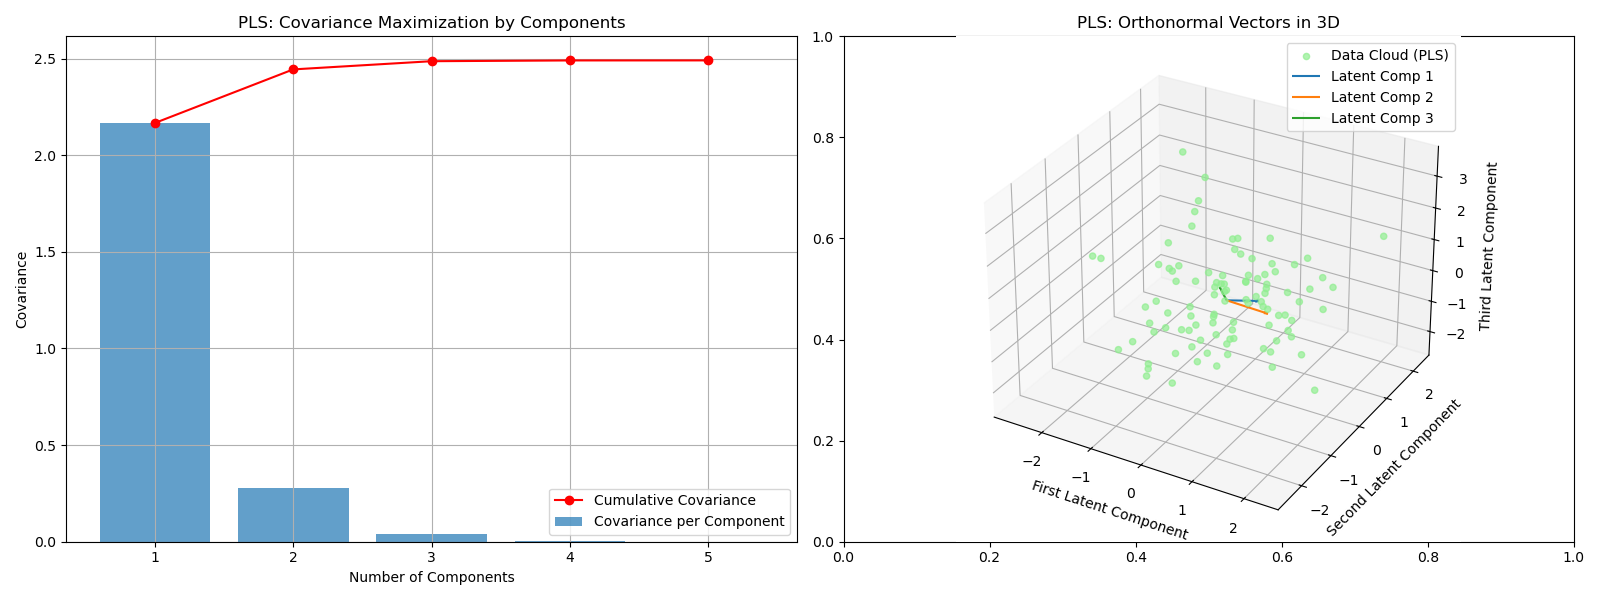
\includegraphics[width=0.9\textwidth]{PLS_Selected_Analysis.png}
    \caption{Partial Least Squares (PLS) Analysis Results}
    \label{fig:PLS_analysis}
\end{figure}

\paragraph {Mathematical Formulation} \ \

PLS constructs \textbf{latent variables (LVs)} as linear combinations of the original predictors:
\begin{equation}
T = XW, \quad U = YQ
\end{equation}
where:
\begin{itemize}
    \item \( T \) and \( U \) are the latent variables (score matrices) for \( X \) and \( Y \), respectively,
    \item \( W \) and \( Q \) are the weight (loading) matrices that transform \( X \) and \( Y \) into the latent space.
\end{itemize}

PLS selects components by maximizing the covariance between \( XW \) and \( YQ \), ensuring that the extracted components remain highly predictive of the response:
\begin{equation}
W = \arg\max_W \operatorname{cov}(XW, Y)
\end{equation}

The final regression model is then expressed in terms of these components:
\begin{equation}
Y = T \delta + \epsilon
\end{equation}
where \( \delta \) represents the regression coefficients for the latent variables.

\paragraph {Bias-Variance Tradeoff in PLS} \ \

Like PCR, PLS reduces variance by using only the first k components. However, PLS retains predictive power better than PCR because it selects components based on their relevance to Y. 

Extracting first \( k \) PLS components:
\begin{equation}
T_k = XW_k
\end{equation}
where \(W_k \) contains the first \( k \) PLS weight vectors that capture the most covariance between \( X \) and \( Y \) (Figure 2).

Estimating regression coefficients in the latent space:
 \begin{equation}
\hat{\delta_k} = (T_k^T T_k)^{-1} T_k^T Y
\end{equation}

The final regression coefficient in the original space is:
\begin{equation}
\hat{\beta}_{\text{PCR}} = W_k \hat{\delta_k} 
\end{equation}

After substitution we have:
\begin{equation}
\hat{\beta}_{\text{PCR}} = W_k (W_k^T X^T X W_k)^{-1} W_k^T X^T Y
\end{equation}

In the case when all \(p \) components are used, i.e. \(k = p \), we can simplify \(\hat{\beta}_{\text{PCR}} \) and we have:
\begin{equation}
\hat{\beta}_{\text{PLS}} = (X^T X)^{-1} X^T Y = \hat{\beta}_{\text{OLS}} 
\end{equation}
where fewer components lead to lower variance but higher bias. This mechanism prevents overfitting, particularly in high-dimensional settings.

Partial Least Squares Regression offers a robust alternative to standard regression techniques by integrating dimensionality reduction with predictive modeling. Compared to PCR, PLS is a supervised approach, ensuring that the extracted components remain relevant for prediction. This makes PLS an effective tool for applications where both dimensionality reduction and accurate predictions are required.

It is important to clarify that Principal Component Regression (PCR) and Partial Least Squares (PLS) are not feature selection techniques in the traditional sense. Unlike methods such as LASSO or stepwise regression, which explicitly remove irrelevant predictors by setting some regression coefficients to zero, both PCR and PLS transform the original predictor space into a new set of latent variables.

Even though PCR and PLS reduce the dimensionality of the predictor space, they do so by forming linear combinations of all original predictors. This means that each principal component or latent variable still contains information from every predictor in the dataset. Thus, PCR and PLS do not eliminate variables but instead project them into a lower-dimensional space where multicollinearity is mitigated, and variance is better controlled.

\paragraph {NIPALS Algorithm} \ \

Several algorithms exist for computing PLS regression. One of the common, The \textbf{Nonlinear Iterative Partial Least Squares (NIPALS)} algorithm is an iterative approach used to extract PLS components when the number of predictors is very large.

\begin{enumerate}
    \item Initialize \( u = Y[:,1] \), the first column of \( Y \).
    \item Compute the weight vector:
        \begin{equation}
        w = \frac{X^T u}{\|X^T u\|}
        \end{equation}
    \item Compute the latent score vector:
        \begin{equation}
        t = Xw
        \end{equation}
    \item Compute the loading vector:
        \begin{equation}
        p = \frac{X^T t}{t^T t}
        \end{equation}
    \item Compute the regression coefficient:
        \begin{equation}
        b = \frac{u^T t}{t^T t}
        \end{equation}
    \item Deflate \( X \) and \( Y \):
        \begin{equation}
        X = X - tp^T, \quad Y = Y - btq^T
        \end{equation}
    \item Repeat the process until convergence.
\end{enumerate}

We would like to note that the NIPALS algorithm used in Partial Least Squares (PLS) shares structural similarities with the Gram-Schmidt process, as both iteratively construct an orthonormal basis through projection and deflation. However, their objectives differ: Gram-Schmidt is an unsupervised linear algebra technique that orthonormalizes column vectors without considering an external target, whereas NIPALS is a supervised method that builds an orthonormal basis of latent variables to maximize covariance with the response variable \( Y \). While both methods ensure orthogonality at each step, NIPALS deflates both \( X \) and \( Y \) after extracting each latent variable, progressively focusing on predictive directions. This key difference makes PLS more powerful than Principal Component Regression (PCR), as it selects components that are not just orthogonal but also relevant for prediction. In essence, NIPALS can be viewed as a Gram-Schmidt-like process adapted for regression, optimizing feature extraction for predictive accuracy rather than just mathematical convenience.

\paragraph {SIMPLS Algorithm} \ \

An alternative to NIPALS is the SIMPLS (Statistically Inspired Modification of PLS) algorithm, which extracts PLS components without iterative deflation, making it computationally more efficient.

\begin{enumerate}
    \item Compute the covariance matrix:
        \begin{equation}
        S = X^T Y
        \end{equation}
    \item Extract the first singular vector \( r_1 \) from SVD of \( S \).
    \item Compute the score vector:
        \begin{equation}
        t_1 = Xr_1
        \end{equation}
    \item Compute the loading:
        \begin{equation}
        p_1 = X^T t_1 / (t_1^T t_1)
        \end{equation}
    \item Compute the regression coefficient:
        \begin{equation}
        b_1 = (t_1^T Y) / (t_1^T t_1)
        \end{equation}
    \item Deflate the covariance matrix:
        \begin{equation}
        S = S - r_1 (r_1^T S)
        \end{equation}
    \item Repeat for additional components.
\end{enumerate}

SIMPLS is preferred when computational efficiency is a concern, especially for very large datasets. Both methods produce the same final PLS regression coefficients, but their computation methods differ.

\subsection{Selection of the Optimal Number of Components in PCR and PLS}
A crucial aspect of applying PCR and PLS effectively is determining the appropriate number of components (\( k \)) to retain (Figure 2). Selecting too few components may result in underfitting, where important predictive information is lost. Conversely, retaining too many components can lead to overfitting, reducing the generalization ability of the model. In this section we will consider several methods for selecting the optimal number of components in PCR and PLS.

\paragraph {Elbow Method} \ \

The Elbow Method is widely used for selecting the optimal number of components in both Principal Component Regression (PCR) and Partial Least Squares (PLS). The method involves plotting a performance metric—such as cumulative explained variance for PCR or cumulative explained covariance for PLS—against the number of components (Figures 1 and 2). The optimal number of components is chosen at the "elbow point", where the marginal gain in variance or covariance explained diminishes significantly.

In Principal Component Regression (PCR), component selection is based on Principal Component Analysis (PCA), which transforms the original predictor space into a set of orthogonal components that explain the variance in \( X \). Since PCR does not consider the response variable \( Y \) in component selection, it relies on the cumulative explained variance of the predictors.

Mathematically, the proportion of variance explained by the first \( k \) principal components is given by:
\begin{equation}
\text{Explained Variance}(k) = \frac{\sum_{i=1}^{k} \lambda_i}{\sum_{i=1}^{p} \lambda_i}
\end{equation}
where \( \lambda_i \) are the eigenvalues of the covariance matrix \( X^T X \), which correspond to the variances captured by each principal component.

The selection of \( k \) is determined by identifying the "elbow point" on the cumulative variance plot. This is the point where adding more components results in a negligible increase in explained variance. In practical applications, a commonly used threshold is:
\begin{equation}
\sum_{i=1}^{k} \lambda_i \geq 0.95 \sum_{i=1}^{p} \lambda_i
\end{equation}
indicating that at least 95\% of the total variance in \( X \) has been retained.

Unlike PCR, which selects components based solely on variance in \( X \), Partial Least Squares (PLS) extracts components that maximize the covariance between \( X \) and \( Y \). Therefore, the Elbow Method in PLS is based on the cumulative explained covariance rather than variance.

For PLS, we define the cumulative explained covariance as:
\begin{equation}
\text{Explained Covariance}(k) = \frac{\sum_{i=1}^{k} \text{Cov}(t_i, y)^2}{\sum_{i=1}^{p} \text{Cov}(t_i, y)^2}
\end{equation}
where \( t_i \) are the latent variables obtained from PLS, which are linear combinations of the original predictors.

Similar to PCR, the "elbow point" is identified on the cumulative covariance plot, marking the point beyond which additional components contribute minimally to predictive power. The typical threshold for PLS component selection is:
\begin{equation}
\sum_{i=1}^{k} \text{Cov}(t_i, y)^2 \geq 0.90 \sum_{i=1}^{p} \text{Cov}(t_i, y)^2
\end{equation}
indicating that at least 90\% of the total covariance between \( X \) and \( Y \) is captured by the first \( k \) components.

The Elbow Method provides a simple yet effective means of selecting \( k \), but its effectiveness depends on the dataset. If the "elbow" is not clearly visible, alternative methods such as the \textbf{Needle Algorithm} or \textbf{Cross-Validation (CV)} should be used to refine component selection.

\paragraph {Needle Algorithm} \ \

The Needle Algorithm is an alternative method for determining the optimal number of components, which provides a formalized way of detecting the point beyond which additional components contribute negligibly to the model. It is particularly useful when the variance or covariance decay is gradual, making the elbow point ambiguous.

In PCR, The Needle Algorithm identifies \( k \) by examining the second derivative of the cumulative explained variance function. Mathematically, the proportion of variance explained by the first \( k \) components is:
\begin{equation}
\text{Explained Variance}(k) = \frac{\sum_{i=1}^{k} \lambda_i}{\sum_{i=1}^{p} \lambda_i}
\end{equation}
where \( \lambda_i \) are the eigenvalues of \( X^T X \). 

The \textbf{Needle Criterion} is defined as:
\begin{equation}
\Delta_k = \lambda_k - \lambda_{k+1}
\end{equation}
\begin{equation}
\text{Relative Gain}(k) = \frac{\Delta_k}{\sum_{i=1}^{k} \lambda_i}
\end{equation}

The optimal \( k \) is determined when the relative gain in explained variance falls below a predefined threshold \( \epsilon \), typically around \( 1\% \):
\begin{equation}
\frac{\lambda_k - \lambda_{k+1}}{\sum_{i=1}^{k} \lambda_i} < \epsilon
\end{equation}
This ensures that additional components do not contribute meaningfully to variance retention.

For PLS, the Needle Algorithm follows the same principle but is applied to the explained covariance between \( X \) and \( Y \) instead of variance in \( X \). The proportion of covariance explained by the first \( k \) components is given by:
\begin{equation}
\text{Explained Covariance}(k) = \frac{\sum_{i=1}^{k} \text{Cov}(t_i, y)^2}{\sum_{i=1}^{p} \text{Cov}(t_i, y)^2}
\end{equation}
where \( t_i \) are the latent variables extracted by PLS.

The Needle Criterion for PLS is:
\begin{equation}
\Delta_k = \text{Cov}(t_k, y)^2 - \text{Cov}(t_{k+1}, y)^2
\end{equation}
\begin{equation}
\text{Relative Gain}(k) = \frac{\Delta_k}{\sum_{i=1}^{k} \text{Cov}(t_i, y)^2}
\end{equation}

As in PCR, the optimal \( k \) is found when the relative gain in explained covariance drops below a predefined threshold \( \epsilon \):
\begin{equation}
\frac{\text{Cov}(t_k, y)^2 - \text{Cov}(t_{k+1}, y)^2}{\sum_{i=1}^{k} \text{Cov}(t_i, y)^2} < \epsilon
\end{equation}
Typically, \( \epsilon \) is set to 1\% to 2\%, ensuring that only significant components contributing to the prediction of \( Y \) are retained.

The Needle Algorithm provides a more formal alternative to the Elbow Method, particularly in cases where variance or covariance decays smoothly without a clear "elbow point".

\paragraph {Cross-Validation} \ \

Cross-Validation (CV) is a data-driven approach to selecting the optimal number of components. Unlike the Elbow Method or the Needle Algorithm, which focus on variance or covariance retention, CV directly evaluates the predictive performance of the model by minimizing the generalization error. This ensures that the selected number of components leads to the best tradeoff between bias and variance.

In PCR, the key challenge is to determine how many principal components (\( k \)) should be retained to ensure strong predictive performance. Since PCR does not use the response variable \( Y \) when selecting components, cross-validation is crucial in identifying the point where including additional components no longer improves prediction accuracy.

The procedure for selecting \( k \) via CV follows these steps:
\begin{enumerate}
    \item Split the dataset into \( K \) \textbf{folds} (typically \( K = 5 \) or \( K = 10 \)).
    \item For each fold, fit the \textbf{PCR model} using the first \( k \) principal components and compute the prediction error on the held-out data.
    \item Compute the \textbf{Cross-Validation Mean Squared Error (CV-MSE)} for each \( k \):
    \begin{equation}
    \text{CV-MSE}(k) = \frac{1}{n} \sum_{i=1}^{n} (y_i - \hat{y}_{-i,k})^2
    \end{equation}
    where \( \hat{y}_{-i,k} \) is the prediction for the \( i \)-th observation using a model trained without that observation and with \( k \) components.
    \item Select \( k^* \) that minimizes \(\text{CV-MSE}(k)\):
    \begin{equation}
    k^* = \arg\min_k \text{CV-MSE}(k)
    \end{equation}
\end{enumerate}

Since PCR selects principal components without considering \( Y \), CV ensures that the selected components contribute to predictive accuracy rather than just maximizing variance in \( X \).

Unlike PCR, PLS constructs components that maximize the covariance between \( X \) and \( Y \). Thus, CV in PLS plays a slightly different role: it helps determine the number of latent variables that maximize predictive accuracy.

The CV procedure for PLS follows the same general steps as in PCR:
\begin{enumerate}
    \item Split the dataset into \( K \) \textbf{folds}.
    \item For each fold, fit the \textbf{PLS model} using the first \( k \) latent variables and compute the prediction error on the held-out data.
    \item Compute the \textbf{CV-MSE} for each \( k \):
    \begin{equation}
    \text{CV-MSE}(k) = \frac{1}{n} \sum_{i=1}^{n} (y_i - \hat{y}_{-i,k})^2
    \end{equation}
    \item Select \( k^* \) that minimizes \(\text{CV-MSE}(k)\):
    \begin{equation}
    k^* = \arg\min_k \text{CV-MSE}(k)
    \end{equation}
\end{enumerate}

Since PLS incorporates \( Y \) in selecting components, it is expected to achieve lower optimal \( k^* \) and lower CV-MSE compared to PCR for a given dataset, particularly when \( X \) and \( Y \) are highly correlated.

Cross-validation is the most rigorous method for selecting $k$, but it comes with some practical considerations. One major concern is computational cost, as it requires training multiple models for different values of $k$ across several folds, making the process resource-intensive. Additionally, cross-validation plays a crucial role in managing the bias-variance tradeoff. Smaller values of $k$ tend to introduce higher bias, whereas larger values lead to increased variance. The goal is to find an optimal balance between these two factors. In practice, common choices for $k$ are 5 or 10. While opting for a smaller $k$ can reduce computation time, a larger $k$ generally provides a more reliable error estimate.

The choice of \( k \) should be guided by a combination of these methods, balancing the need for variance retention and predictive accuracy. In empirical applications, cross-validation is typically preferred due to its ability to optimize for prediction error directly, therefore CV is applied in our simulations and empirical estimation.

\section{Simulation Study}

The goal of this simulation study is to evaluate the performance of Principal Component Regression (PCR) and Partial Least Squares (PLS) across different data-generating scenarios, focusing on their predictive accuracy, robustness, and bias-variance trade-offs in high-dimensional settings. Given the common challenges posed by multicollinearity and high-dimensional predictor spaces, we employ a Monte Carlo simulation framework to systematically analyze the behavior of these methods under varying feature dependencies. Simulation study is structured around three distinct setups:

\begin{enumerate}
    \item \textbf{Classical Data (No Multicollinearity)}: Predictors are independently sampled from a normal distribution, ensuring no multicollinearity.
    \item \textbf{Moderate Multicollinearity}: The predictor matrix consists of a set of base features along with additional highly correlated features, introducing a controlled level of dependence.
    \item \textbf{Severe Multicollinearity (Low Observations)}: The predictors exhibit strong correlations, with only a subset contributing to the response variable. This setup mimics scenarios where multicollinearity is extreme and sample size is limited, testing the methods' ability to extract meaningful structure from highly dependent data.
\end{enumerate}

To assess performance, we first apply PCR by performing Principal Component Analysis (PCA) on the predictor matrix and selecting the optimal number of components via \( k \)-fold cross-validation, minimizing the Root Mean Squared Error (RMSE) of prediction. Using these selected components, an Ordinary Least Squares (OLS) regression model is fitted, and predictive accuracy is evaluated through RMSE and Mean Squared Error (MSE). Additionally, we analyze the bias-variance trade-off of the coefficient estimates, comparing them to standard OLS results to quantify the extent of regularization. 

Similarly, for PLS, we employ the Nonlinear Iterative Partial Least Squares (NIPALS) algorithm to extract latent components, selecting the optimal number via cross-validation to balance model complexity and predictive power. A PLS regression model is then fitted to the transformed predictor matrix, with performance assessed through RMSE, MSE, and coefficient stability. 

To ensure the asymptotic validity of our findings, we conduct a Monte Carlo simulation, generating 1000 datasets for each three setups to evaluate the stability of coefficient estimates, their bias-variance decomposition, and how these methods perform in large-sample scenarios. By systematically comparing PCR, PLS, and OLS across these conditions, we gain deeper insights into their relative advantages and limitations in high-dimensional regression problems.


\subsection{Data Description}
The dataset for each scenario is generated as follows:

\paragraph{Classical Data (No Multicollinearity)}
\begin{itemize}
    \item The predictor matrix \( X \) consists of \( n = 200 \) observations and \( p = 10 \) predictors, generated independently from a standard normal distribution:
    \[ X \sim \mathcal{N}(0, I_p) \]
    \item The response variable follows:
    \[ Y = X \beta + \epsilon, \quad \epsilon \sim \mathcal{N}(0, 0.1) \]
    \item All 10 predictors are actively used to generate \( Y \).
\end{itemize}

\paragraph{Moderate Multicollinearity}
\begin{itemize}
    \item The dataset contains \( n = 200 \) observations and \( p = 10 \) predictors.
    \item A \textbf{base predictor matrix} \( X_{\text{base}} \) is generated as:
    \[ X_{\text{base}} \sim \mathcal{N}(0, I) \]
    \item Additional features are constructed as:
    \[ X_{\text{extra}} = X_{\text{base}} + \eta, \quad \eta \sim \mathcal{N}(0, 0.1) \]
    where \( \eta \) introduces correlation between the predictors.
    \item The final predictor matrix is formed by concatenation:
    \[ X = [X_{\text{base}}, X_{\text{extra}}] \]
    \item The response variable is generated as:
    \[ Y = X \beta + \epsilon, \quad \epsilon \sim \mathcal{N}(0, 1.0) \]
    \item All 10 predictors are actively used to generate \( Y \).
\end{itemize}

\paragraph{Severe Multicollinearity (Low Observations)} \ \

\begin{itemize}

    \item The dataset contains only \( n = 40 \) observations and \( p = 10 \) predictors, creating a scenario where the number of observations is significantly lower than in previous setups.
    \item A base predictor matrix is generated as:
    \[ X_{\text{gen}} \sim \mathcal{N}(0, I) \]
    \item Additional predictors are formed via a linear transformation:
    \[ X_{\text{additional}} = X_{\text{gen}} W + \mathcal{N}(0, 0.1) \]
    where \( W \) represents a randomly generated weight matrix, introducing strong collinearity among predictors.
    \item The response variable follows:
    \[ Y = X \beta + \epsilon, \quad \epsilon \sim \mathcal{N}(0, 1.0) \]
    \item Importantly, only \textbf{three} of the 10 predictors actively contribute to generating \( Y \), while the remaining seven are purely collinear noise variables.
    
\end{itemize}

In the severe multicollinearity scenario, the reduction in the number of observations relative to the number of predictors amplifies the risk of overfitting and instability in regression models. Furthermore, since only three predictors actively contribute to the response variable while the remaining seven are collinear noise, methods like PCR and PLS must effectively distinguish between relevant and redundant information. 

PCR, which selects components based on variance, may retain principal components influenced by multicollinear features, leading to potential inefficiencies in prediction. Conversely, PLS, which maximizes covariance with \( Y \), is expected to perform better in identifying relevant predictors, thus mitigating the negative impact of multicollinearity.

\subsection{Simulation Results: Classical Dataset (No Multicollinearity)}  

In this scenario, the predictors are generated independently, ensuring there is no correlation between them. This setup creates the ideal conditions for Ordinary Least Squares (OLS) regression, which serves as the benchmark for evaluating Principal Component Regression (PCR) and Partial Least Squares (PLS). Our goal is to analyze how these methods perform when no multicollinearity is present and how their behavior changes as the number of components increases.

As expected, OLS performs the best, achieving the lowest Mean Squared Error (MSE) and producing coefficient estimates that closely match the true values. Because there is no multicollinearity, OLS remains unbiased and efficient, making it the optimal estimator in this setting. However, when we apply PCR and PLS, we see a clear difference in how they handle feature selection and regularization.  

Since PCR selects components based purely on variance, it struggles when using only a few components. For instance, with PCR(1) (one principal component), the model captures only a limited portion of the predictor space, leading to high bias. However, as we increase the number of components (PCR(5), PCR(10)), the model recovers more information, reducing bias and approaching OLS-level accuracy. This improvement demonstrates the classic bias-variance trade-off: fewer components introduce higher bias but lower variance, while more components reduce bias at the cost of increasing variance.  

In contrast, PLS finds a balance between bias and variance more efficiently than PCR. Unlike PCR, which selects components based solely on predictor variance, PLS chooses components based on their relationship with the response variable. This allows PLS to extract relevant predictive features even with a small number of components. As a result, PLS with fewer components (e.g., PLS(1), PLS(5)) already provides better coefficient estimates and lower MSE compared to PCR with the same number of components. This suggests that PLS is a more efficient dimensionality reduction method when the goal is to improve prediction accuracy.

The impact of component selection is further reflected in the quality of predictions. OLS predictions align almost perfectly with real values, reinforcing its reliability in this scenario. On the other hand, PCR with very few components, such as PCR(1), struggles to capture the full structure of the data, leading to poor predictions and a weaker fit. However, as the number of components increases, the predictions improve significantly, with PCR(10) closely matching the performance of OLS. In comparison, PLS consistently performs well even with fewer components, confirming its ability to extract meaningful features efficiently. This efficiency allows PLS to achieve strong predictive performance while using fewer dimensions than PCR, making it a more robust choice when dimensionality reduction is necessary.

The stability of coefficient estimates also reflects these patterns. OLS estimates remain centered around the true values with minimal variation, confirming that it is an unbiased estimator. PCR, on the other hand, shows greater variability when fewer components are used, and its estimates are further from the true values. However, when enough components are included, PCR estimates stabilize and align with OLS. PLS estimates remain more stable than PCR, even with fewer components, highlighting its advantage in capturing relevant information effectively.

\begin{figure}[H]
    \centering
    \begin{subfigure}{0.32\textwidth}
        \centering
        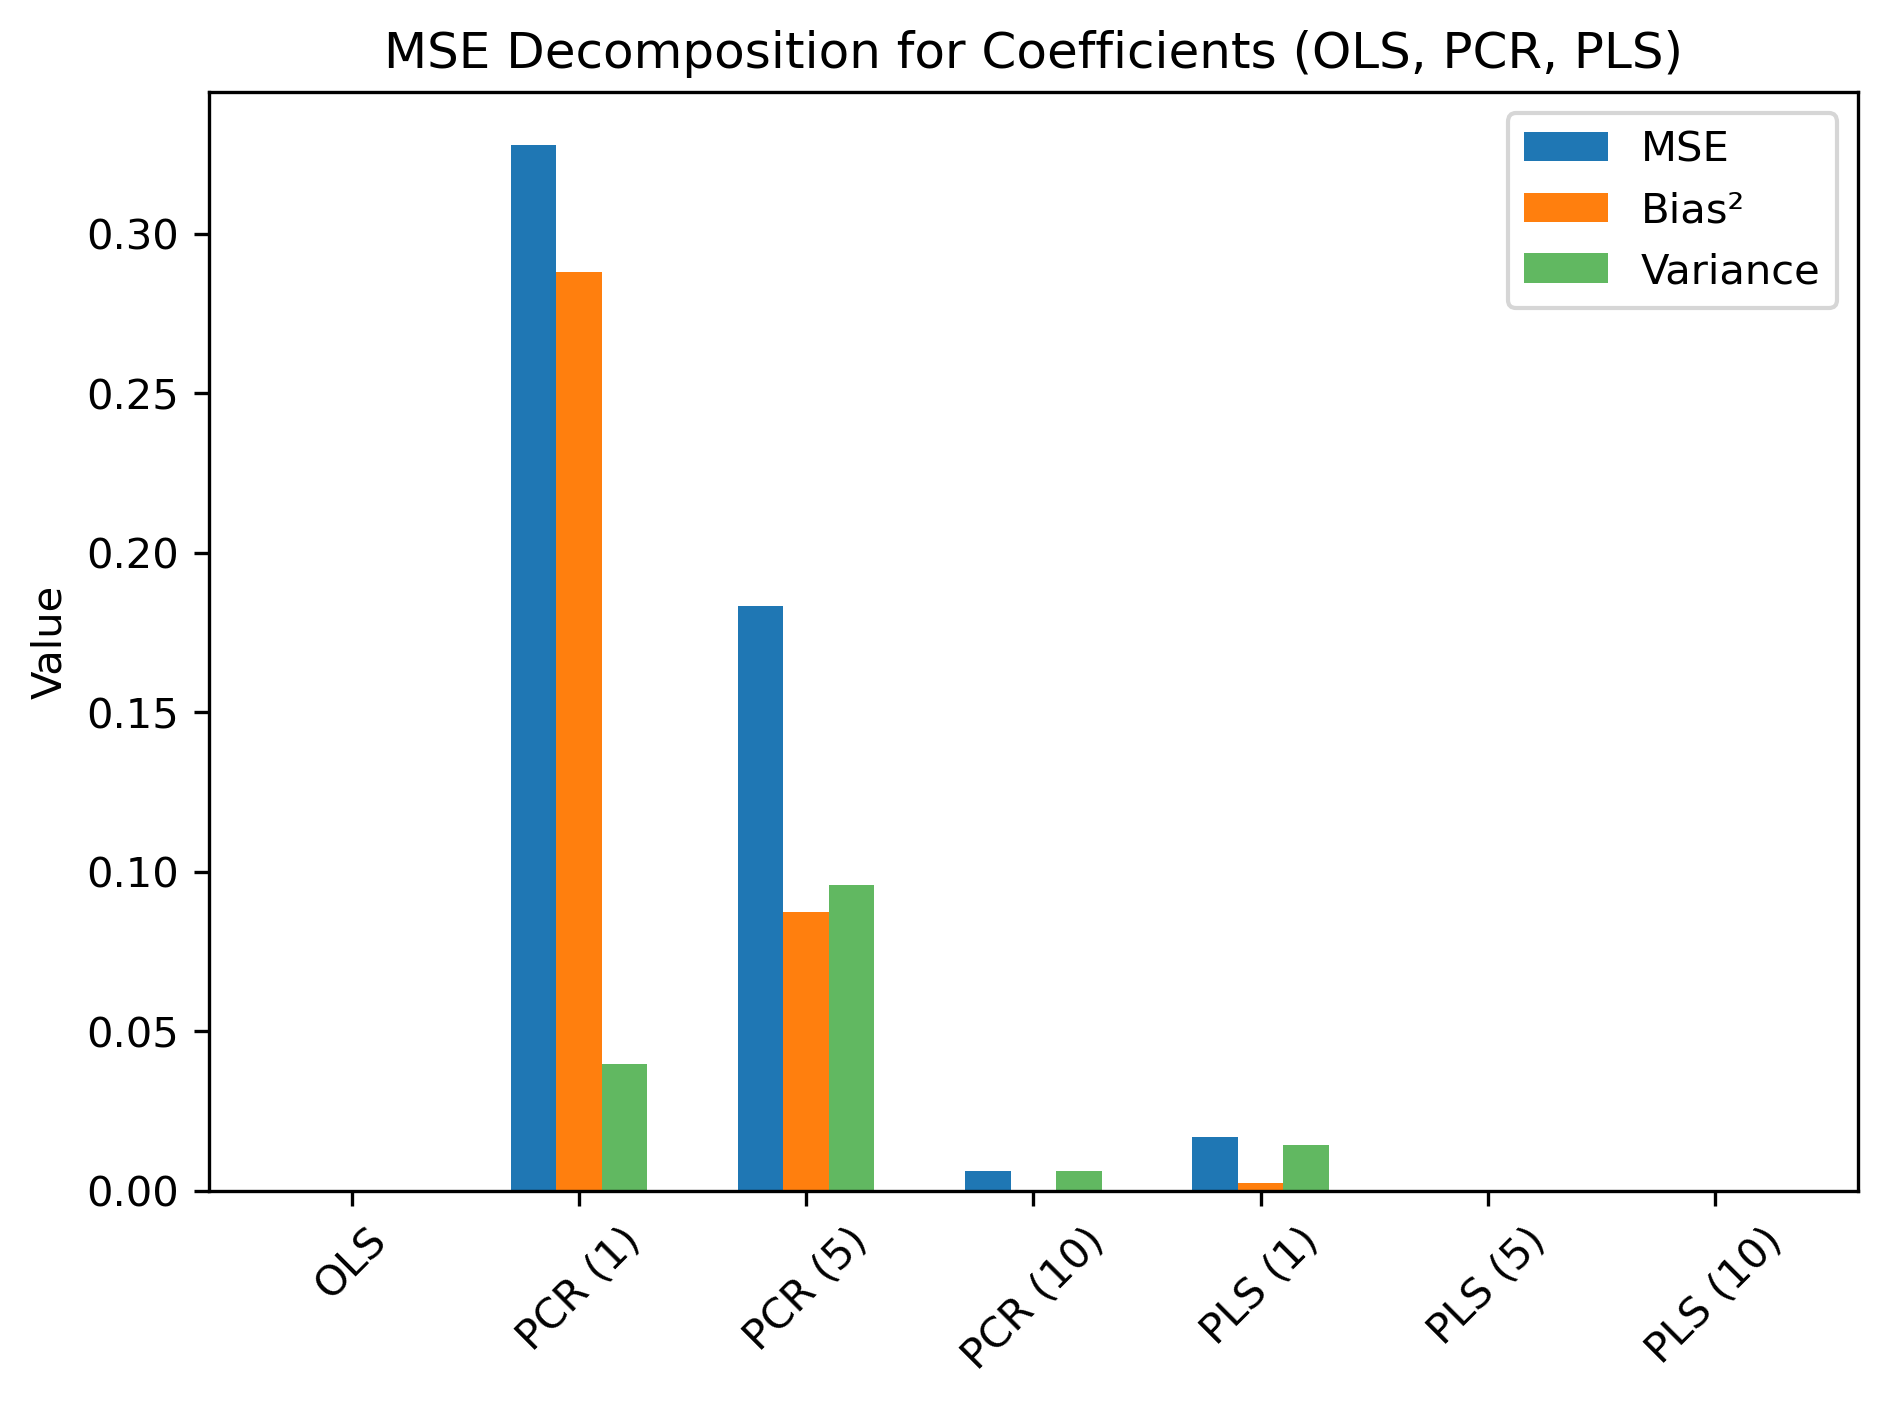
\includegraphics[width=\linewidth]{Fifth_plot.png}
        \caption{Classic Data Analysis}
        \label{fig:Classic_data_analysis}
    \end{subfigure}
    \hfill
    \begin{subfigure}{0.32\textwidth}
        \centering
        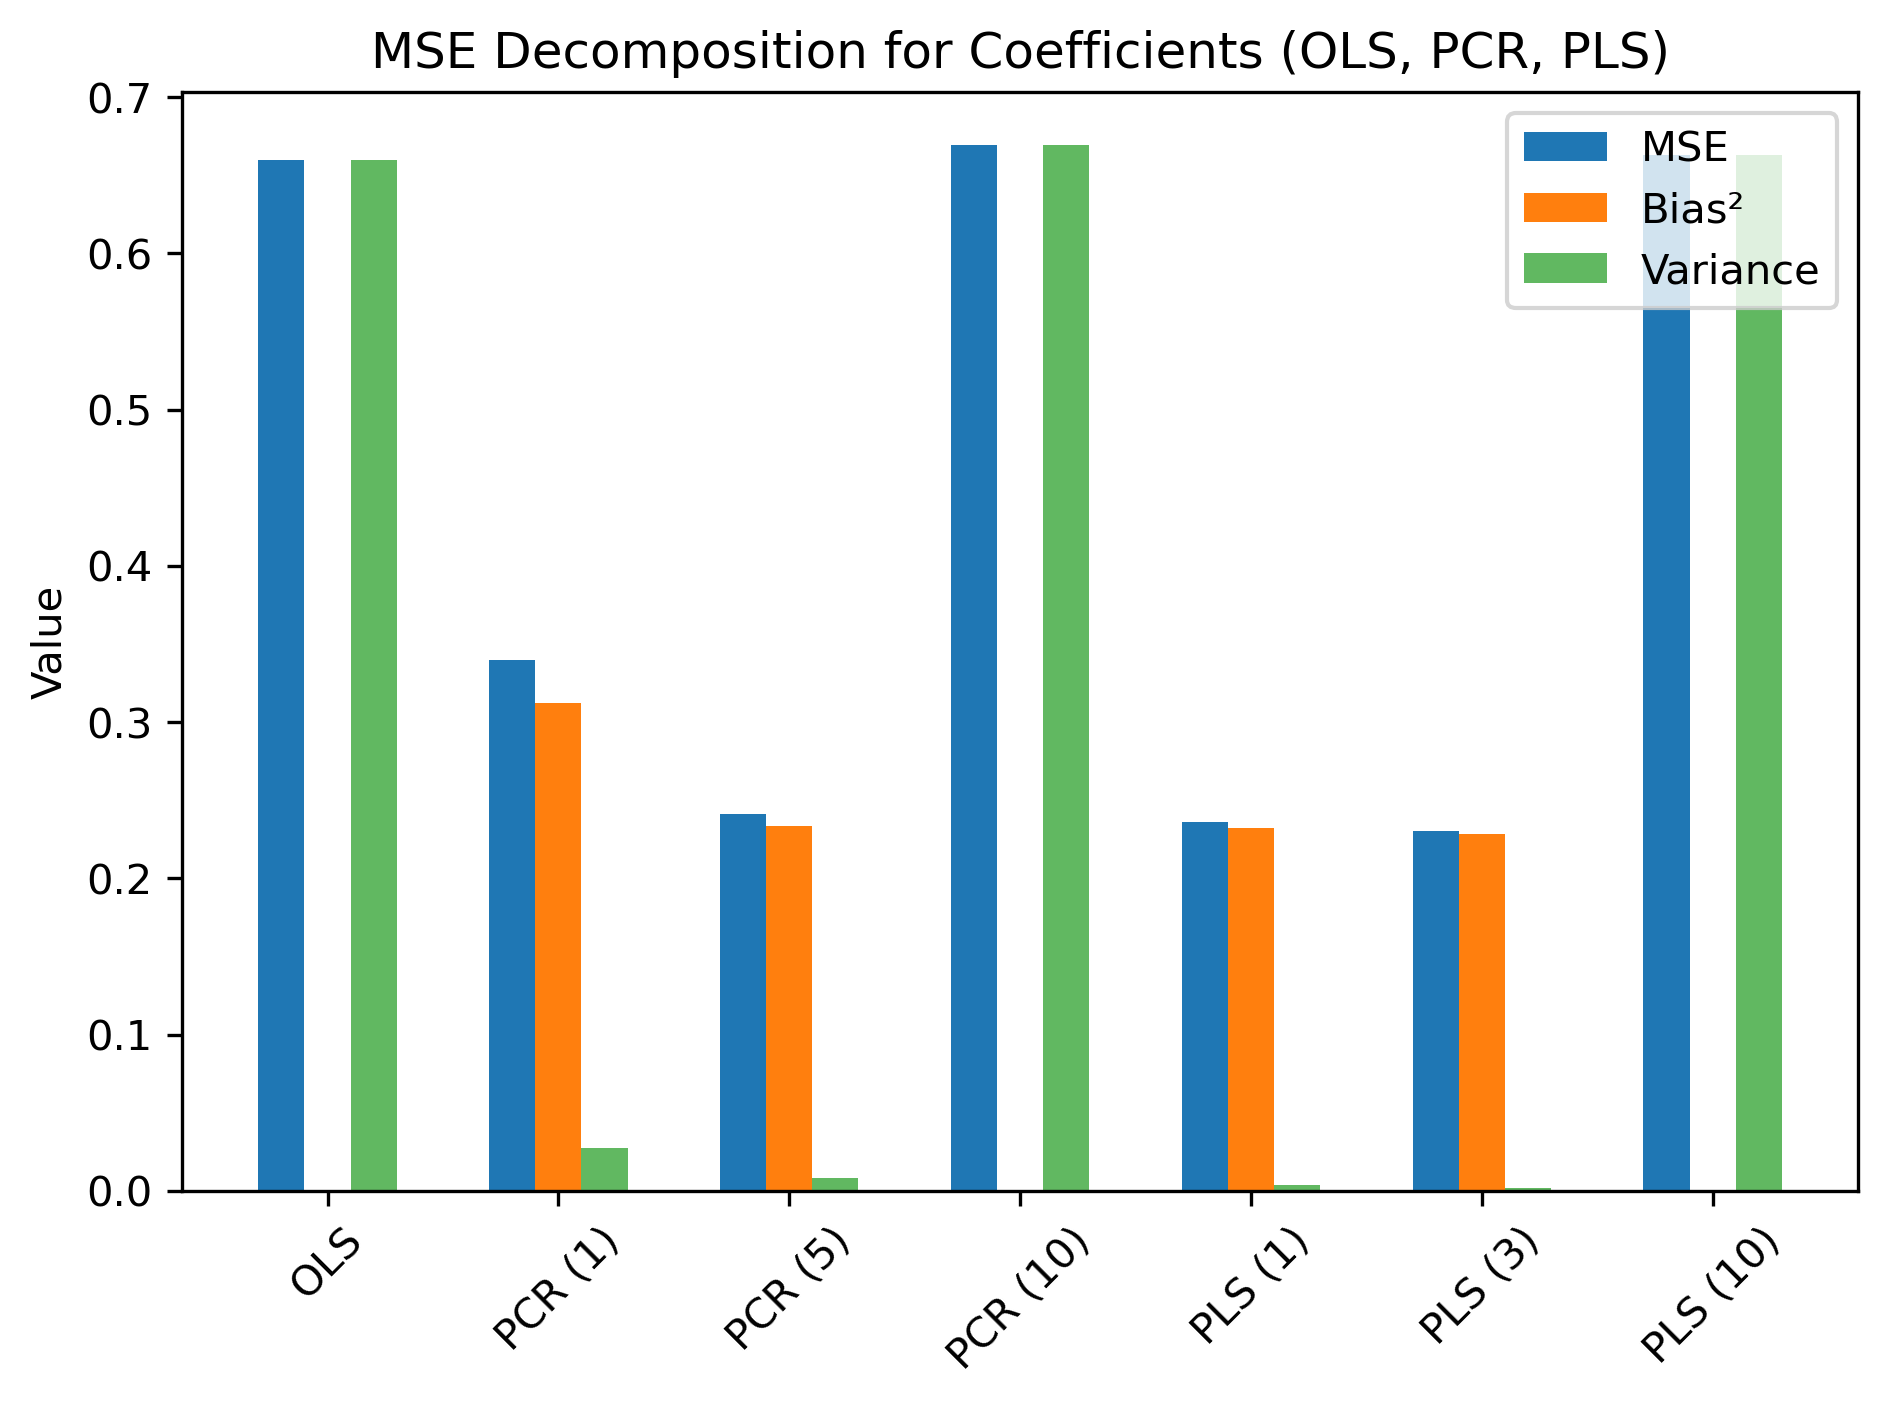
\includegraphics[width=\linewidth]{Fifth_plot_second_simulation.png}
        \caption{Moderate Multicollinearity}
        \label{fig:Moderate_multicollinear_data_analysis}
    \end{subfigure}
    \hfill
    \begin{subfigure}{0.32\textwidth}
        \centering
        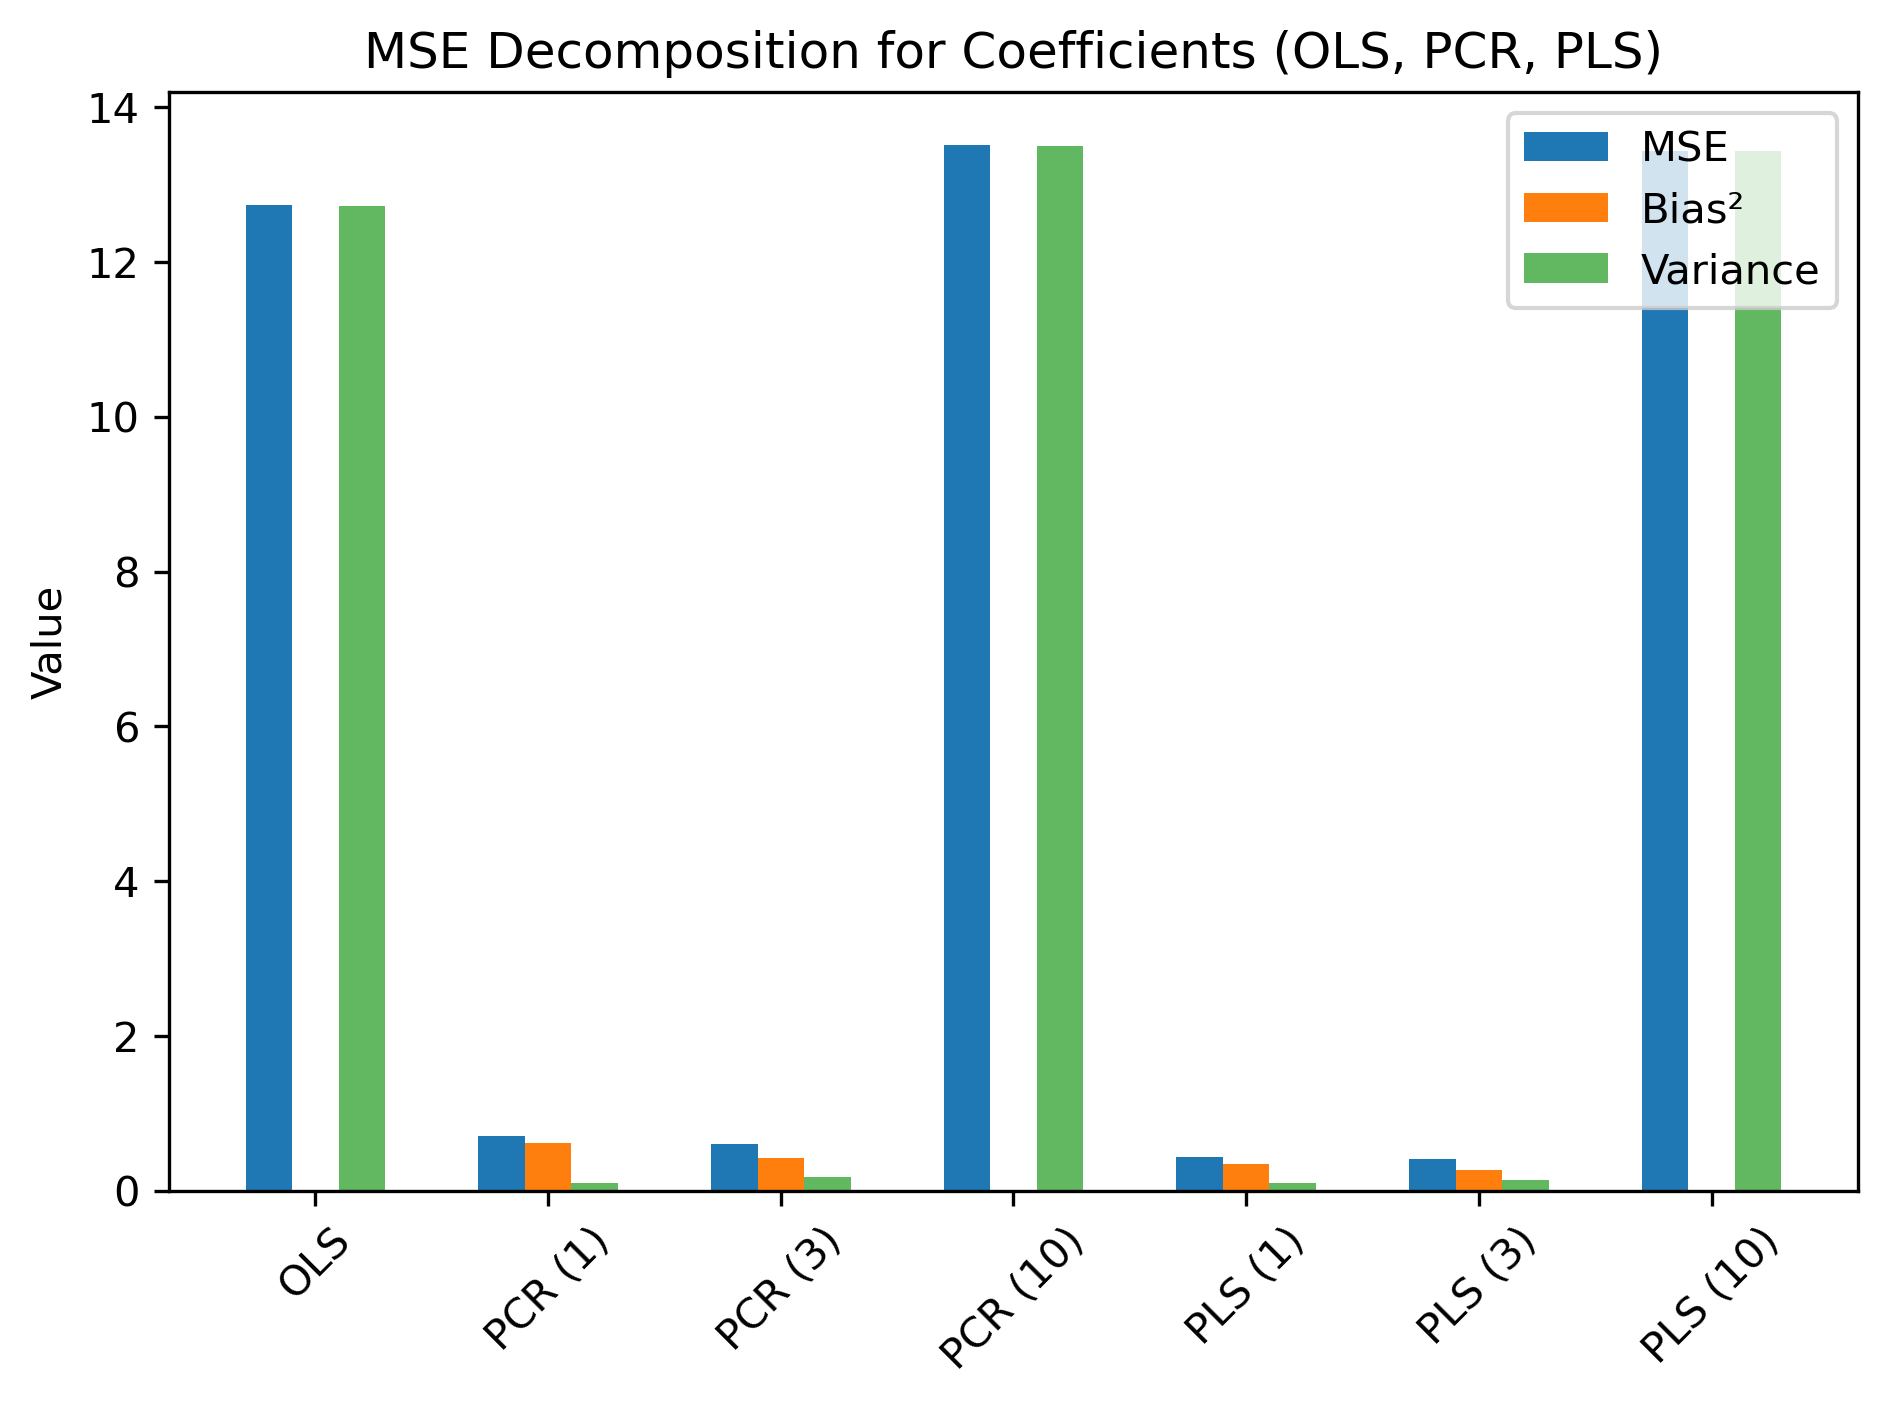
\includegraphics[width=\linewidth]{Fifth_plot_third_simulation.png}
        \caption{Severe Multicollinearity}
        \label{fig:Severe_multicollinear_data_analysis}
    \end{subfigure}
    \caption{Bias-Variance trade-off: OLS, PCR, and PLS for different cases}
    \label{fig:BiasVarianceTradeoff}
\end{figure}

OLS is the best option when there is no multicollinearity, as it provides the most accurate and stable coefficient estimates. PCR requires a sufficient number of components to recover the full predictor space. Using too few components results in high bias and poor predictions, but increasing the number of components improves performance. PLS is more efficient than PCR in selecting relevant features, achieving strong predictive performance with fewer components. The bias-variance trade-off is evident—fewer components lead to high bias (underfitting), while using too many components increases variance (potential overfitting).

This classical dataset serves as a baseline reference, showing how PCR and PLS behave under ideal conditions. The next step is to explore how these methods perform when moderate multicollinearity is introduced, where predictors become correlated and the assumptions of OLS begin to break down.

\subsection{Simulation Results: Moderate Multicollinearity Dataset}  

In this scenario, the predictor variables are moderately correlated, introducing a controlled level of multicollinearity. This setup challenges the assumptions of Ordinary Least Squares (OLS) regression and allows us to assess how Principal Component Regression (PCR) and Partial Least Squares (PLS) handle collinearity and improve prediction performance.

When predictors exhibit moderate multicollinearity, OLS starts to struggle as the variance of coefficient estimates increases. This is evident in the Mean Squared Error (MSE) decomposition, where OLS has a significantly high variance component. While OLS remains unbiased, its estimates become unstable due to the correlated predictors.

PCR mitigates this issue by reducing the predictor space to uncorrelated principal components. However, with too few components (e.g., PCR(1)), the model captures only limited variance, resulting in high bias. As the number of components increases (PCR(5), PCR(10)), bias decreases, and the model performance improves. Nevertheless, PCR does not explicitly use response variable information when selecting components, which can lead to inefficiencies in retaining relevant predictive information.

PLS, in contrast, is designed to extract components that maximize covariance with the response variable. This allows PLS to achieve a better balance between bias and variance with fewer components compared to PCR. Even with a small number of components (e.g., PLS(3)), it outperforms PCR with the same number of components, as it better identifies the underlying structure in the data.

The impact of multicollinearity on model predictions becomes evident when comparing actual vs. predicted values. OLS predictions are less stable due to inflated coefficient variance, leading to fluctuations in its predictive performance. PCR with very few components underfits the data, failing to capture enough variance for accurate predictions. However, as the number of components increases, PCR’s predictions align more closely with actual values, though it still lags behind PLS.

PLS consistently provides a stronger predictive fit, even with fewer components. Its predictions are closer to the true values, demonstrating that selecting components based on their relevance to the response variable improves generalization. This makes PLS a more robust choice when multicollinearity is present.

The stability of coefficient estimates also reflects these patterns. OLS estimates show high variability, confirming its sensitivity to multicollinearity. PCR, when using too few components, exhibits significant bias, whereas with more components, its estimates stabilize. PLS remains more stable than PCR throughout, highlighting its effectiveness in handling multicollinearity.

OLS struggles in the presence of moderate multicollinearity, with high variance in coefficient estimates reducing prediction stability. PCR mitigates multicollinearity but requires enough components to recover essential variance. Selecting too few components results in high bias, while increasing components gradually improves predictions. PLS effectively balances bias and variance, leveraging response-driven component selection to achieve strong predictive performance with fewer components. PLS outperforms PCR in handling multicollinearity, as it selects components that are directly relevant to the response variable rather than relying solely on variance. The bias-variance trade-off remains crucial—too few components lead to underfitting (high bias), whereas too many components can introduce instability.

This dataset highlights the limitations of OLS in correlated predictor settings and demonstrates the advantages of PCR and PLS as alternatives. The next step is to explore how these methods perform under severe multicollinearity, where predictor correlations are extreme, and the number of observations is limited.

\subsection{Simulation Results: Severe Multicollinearity with Low Observations}  

In this scenario, the dataset contains only 40 observations with 10 predictors, where the predictors exhibit strong multicollinearity. The additional predictors are generated via a linear transformation of a base predictor matrix, leading to extreme correlations. Furthermore, only three predictors contribute to the response variable, while the remaining predictors act as redundant noise. This setup presents an extreme case of multicollinearity, making it a challenging setting for regression models.

With severe multicollinearity and a low number of observations, OLS struggles the most. The variance of coefficient estimates becomes excessively high, leading to unstable and unreliable predictions. The MSE decomposition shows that OLS has an extremely high variance component, making it unsuitable for this setting. Even though OLS remains unbiased, its high variance leads to large fluctuations in predictions, reducing its overall reliability.

PCR attempts to mitigate this issue by selecting principal components that capture the most variance. However, when using too few components (e.g., PCR(1) or PCR(3)), the model oversimplifies the predictor space, leading to high bias. As more components are included (e.g., PCR(10)), the model performance improves significantly. PLS, due to its supervised nature, requires fewer components to reach a similar level of accuracy compared to PCR. However, when PCR is given enough components, it also reaches comparable predictive performance. 

At their optimal points, both PCR and PLS still exhibit some level of bias, as the component selection inherently introduces regularization. However, this bias is outweighed by the substantial reduction in variance, leading to a much lower overall MSE compared to OLS. This highlights the key advantage of regularization-based methods: while they sacrifice some degree of unbiasedness, they compensate by stabilizing predictions and significantly improving generalization performance.

The impact of severe multicollinearity on predictions is evident when comparing real vs. predicted values. OLS predictions show substantial instability, reflecting its inability to handle highly correlated predictors in small sample sizes. PCR with very few components underfits the data due to high bias, leading to weak predictive performance. However, as more components are included, PCR predictions gradually improve. PLS, benefiting from its supervised component selection, achieves a strong predictive fit with fewer components. When PCR is allowed to utilize a sufficient number of components, it reaches a similar performance level.

The stability of coefficient estimates also supports these findings. OLS estimates show extreme variability, confirming its inefficiency in this setting. PCR estimates stabilize as more components are included but still suffer from inefficiencies due to noise retention when too few components are used. PLS maintains stable coefficient estimates even with fewer components due to its response-driven selection. However, when the appropriate number of components is selected, both methods achieve comparable stability.

OLS fails to provide reliable estimates in the presence of severe multicollinearity with low observations due to excessive variance in coefficient estimates. PCR helps reduce multicollinearity effects, but selecting too few components results in high bias, while selecting too many components may introduce noise from redundant predictors. PLS, leveraging its supervised nature, achieves strong predictive performance with fewer components. However, when PCR is given enough components, it reaches a similar level of predictive accuracy, making both methods viable solutions depending on the data and modeling constraints.

At their optimal component selections, PCR and PLS remain slightly biased but achieve significantly lower variance compared to OLS, leading to a much lower overall MSE. This reinforces the effectiveness of regularization-based methods in controlling variance and improving model stability, particularly in high-dimensional, low-sample-size settings.

This dataset highlights the extreme limitations of OLS and demonstrates the importance of feature selection and dimensionality reduction in challenging regression problems. Both PCR and PLS emerge as effective methods for handling highly collinear predictors in small datasets, achieving similar results through different mechanisms—PLS using fewer components due to its supervised nature, while PCR requiring slightly more components to reach the same performance.

\section{Analysis of NIR Data: Corn Moisture Prediction Using PLS and PCR}

The dataset used in this study consists of NIR spectra collected from 80 corn samples, measured using the mp5 NIR spectrometer. Each spectrum contains 700 data points recorded in the wavelength range of 2498–1100 nm at 2 nm intervals. The target variable, moisture content, serves as the dependent variable. This dataset and methodology align closely with the results reported in the referenced paper, where similar approaches were applied to corn data. The high-dimensional nature of the spectral data makes this a challenging regression problem, particularly due to the presence of collinearity among the predictor variables.

\begin{figure}[H]
    \centering
    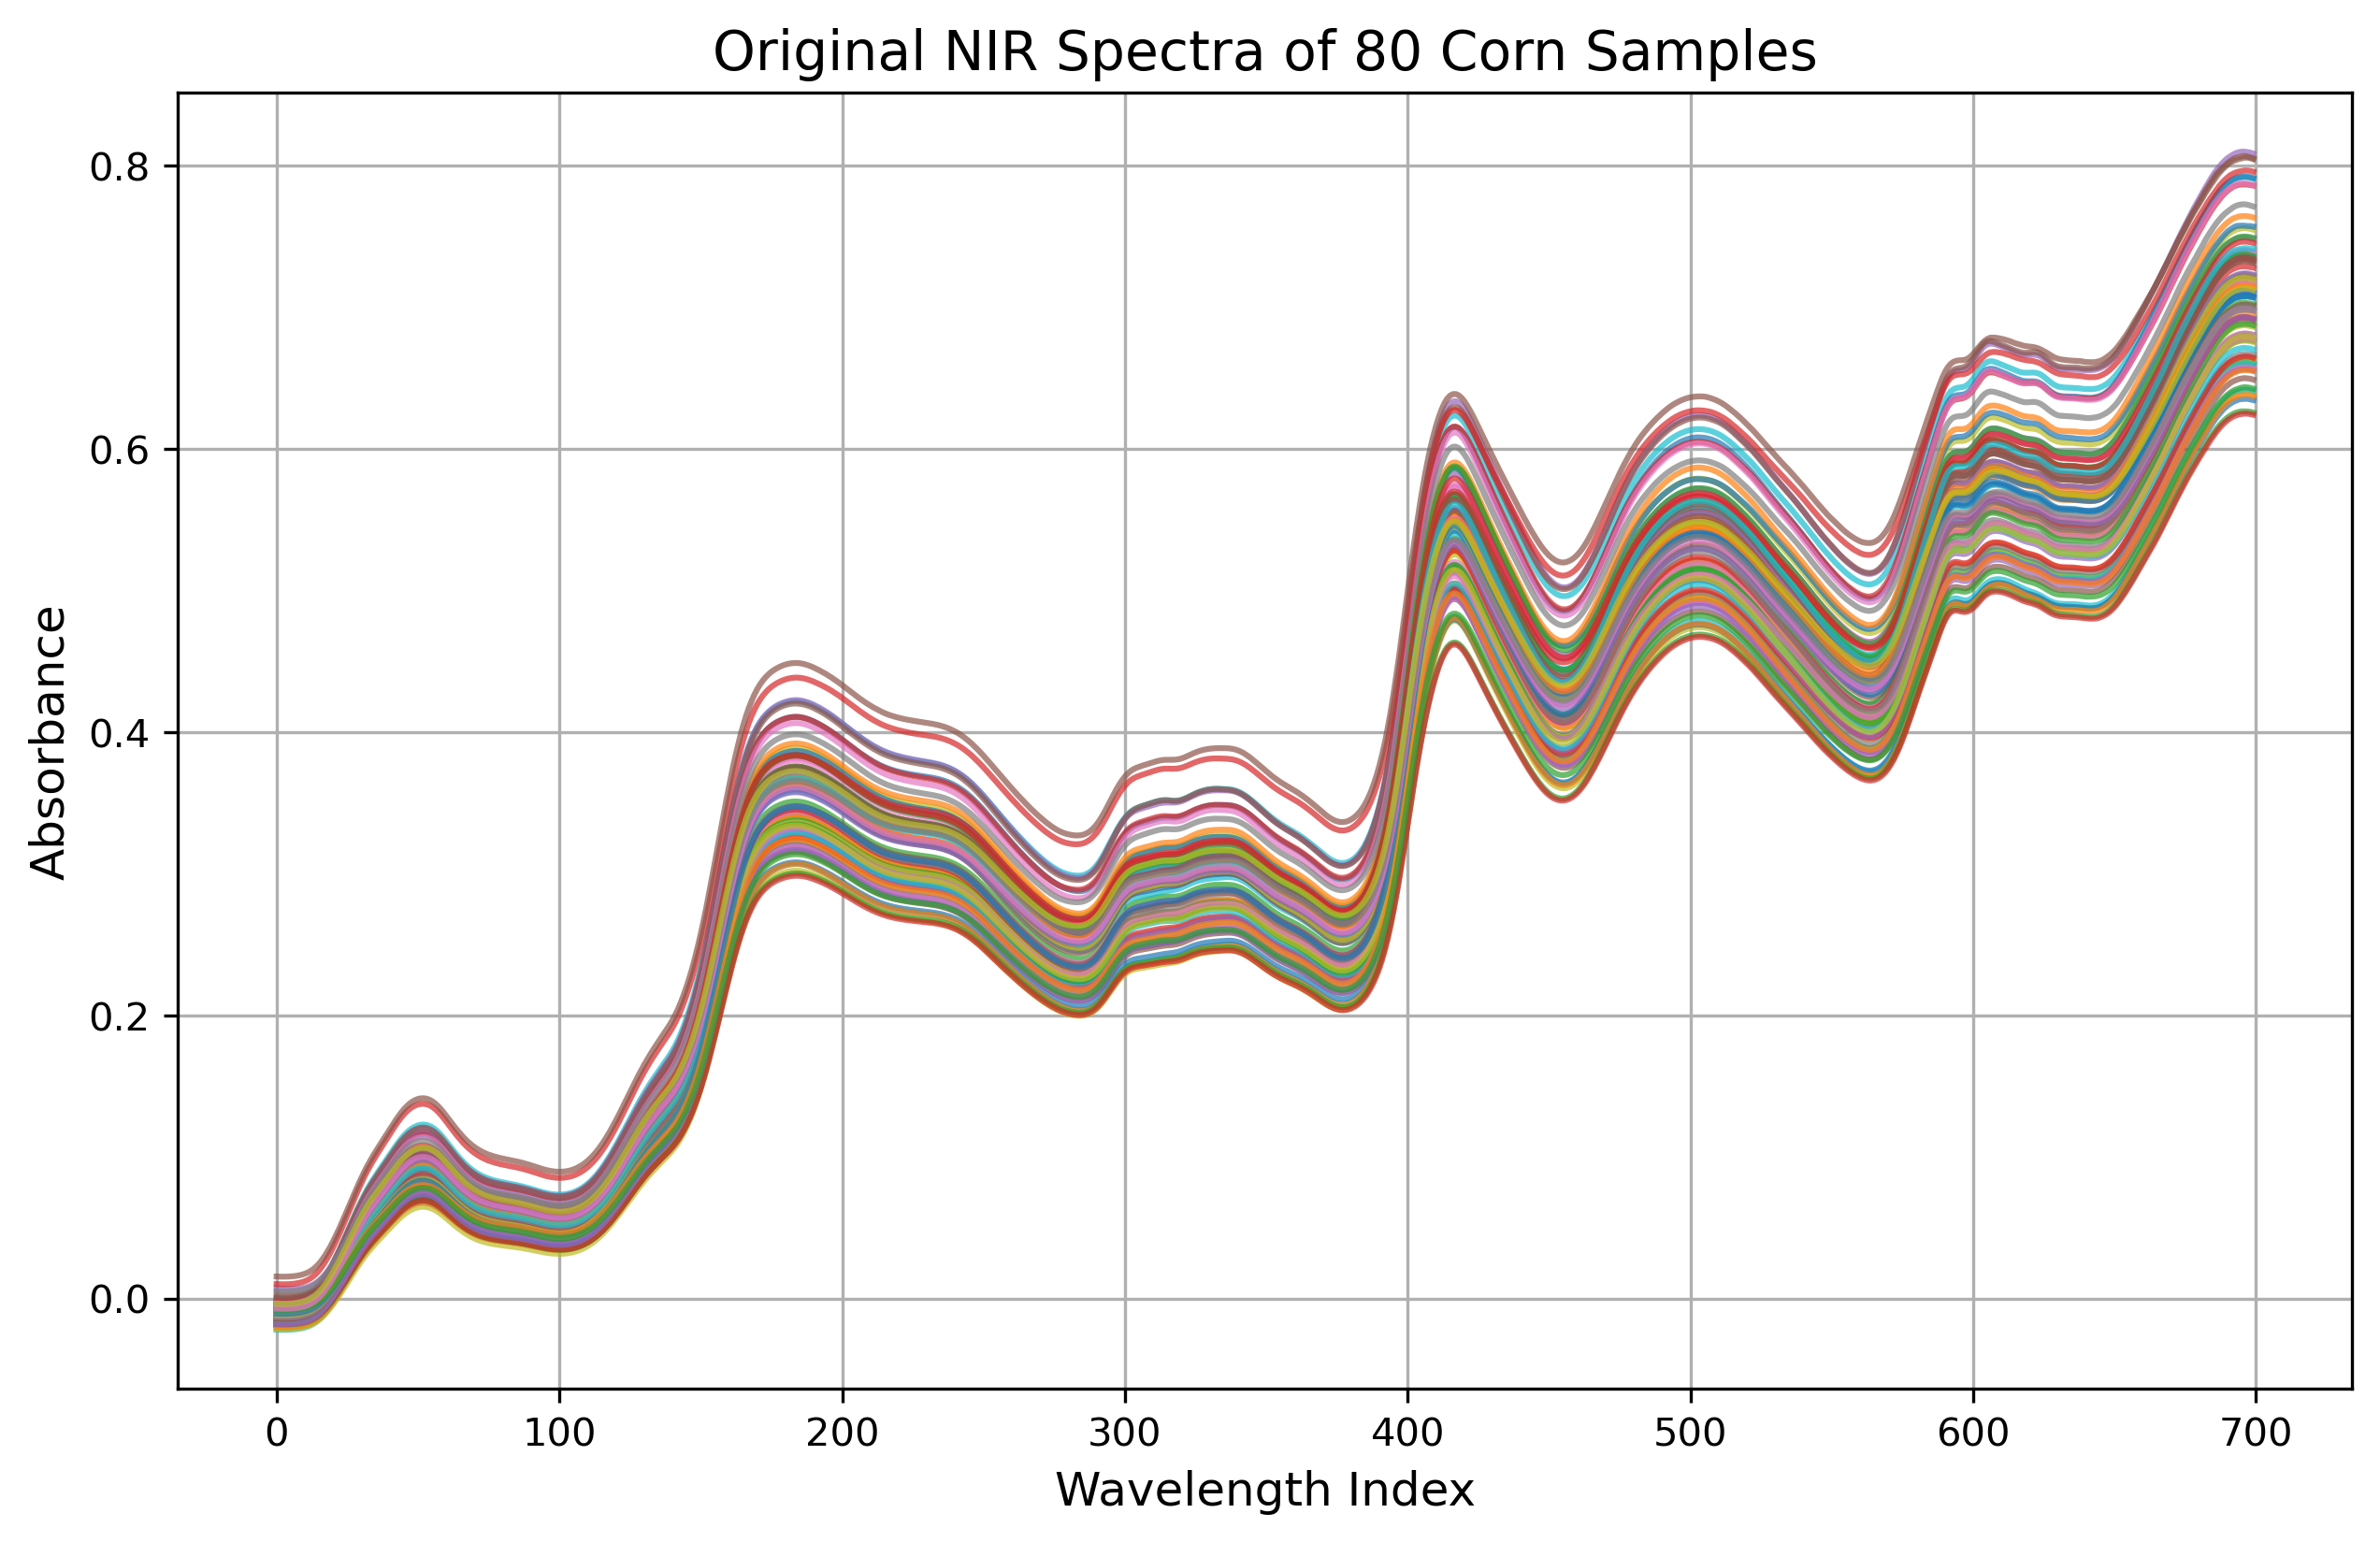
\includegraphics[width=0.9\textwidth]{NIR_first_plot.png}
    \caption{NIR absorption spectra from the Corn Data Set}
    \label{fig:NIR_analysis}
\end{figure}

To evaluate the effectiveness of different regression techniques under this structure, we compare Principal Component Regression (PCR) and Partial Least Squares (PLS). The high multicollinearity present in NIR spectra makes it necessary to use dimensionality reduction techniques. PLS, due to its supervised nature, selects components that maximize covariance with the response variable, while PCR, which is unsupervised, requires a slightly larger number of components to reach a similar level of predictive performance.

A detailed decomposition of Mean Squared Error (MSE) into its bias and variance components illustrates the advantage of using dimensionality reduction. PCR and PLS significantly reduce variance by selecting fewer components, thereby achieving much lower MSE. However, at their optimal component selection points, both PCR and PLS still introduce some bias as a trade-off for reduced variance. This bias, however, is minimal compared to the large variance that would be present if no dimensionality reduction were applied, making PCR and PLS the most suitable approaches for this type of high-dimensional regression problem.

The impact of component selection is further reflected in coefficient estimation. When comparing estimated regression coefficients from PCR and PLS models with varying component counts, it is evident that both methods stabilize the estimates as more components are included. At lower component counts, PLS coefficients align more closely with true values, whereas PCR requires slightly more components to achieve a comparable level of accuracy.

To analyze the stability of coefficient estimates, histograms of the estimated first coefficient provide additional insights. PCR and PLS exhibit much tighter distributions, indicating greater robustness in their estimates. PLS reaches this stability with fewer components, while PCR gradually catches up as more components are included.

Cross-validation is used to determine the optimal number of components for PCR and PLS. The results show a sharp decrease in MSE as the number of components increases, after which the performance stabilizes. PLS achieves its optimal performance with fewer components, while PCR requires slightly more components to reach the same level. Beyond a certain threshold, increasing the number of components leads to overfitting in PLS, causing MSE to rise slightly. This reinforces the importance of selecting the appropriate number of components to balance bias and variance. Meanwhile, PCR is less affected by overfitting due to its unsupervised nature. After reaching its optimal level, PCR performance starts fluctuating instead of consistently increasing with the addition of more components, as it does not rely directly on maximizing covariance with the response variable.

The predictive accuracy of the models is further examined by comparing real and predicted values. PCR and PLS predictions are much closer to the true values, demonstrating their ability to capture meaningful patterns in the data. Since PLS selects components in a way that directly relates to the response variable, it achieves a good predictive fit with fewer components. However, when PCR is allowed to utilize a sufficient number of components, it reaches a similar performance level.

The comparison of actual and fitted values provides additional confirmation of these findings. Both PCR and PLS demonstrate strong agreement between fitted and actual values, highlighting their superior predictive accuracy. PLS, by leveraging response-driven component selection, achieves this accuracy with fewer components, whereas PCR, despite needing slightly more components, still reaches a comparable level of performance.

Overall, this study validates that PCR and PLS provide significantly more reliable estimates for high-dimensional spectral data. Both methods ultimately achieve similar predictive accuracy, but PLS requires fewer components due to its supervised approach, whereas PCR needs slightly more components to reach the same results. The stability of coefficient estimates and predictive performance confirm that both PCR and PLS are highly effective in handling multicollinearity in NIR spectroscopy data. Cross-validation results further reinforce their advantages, showing that regularization through dimensionality reduction is essential for improving model stability and predictive performance. The findings align with previous research demonstrating the bias-variance trade-off in PLS, where increasing the number of latent variables initially reduces bias but eventually leads to overfitting, as evidenced by increasing cross-validation error. In contrast, PCR, being unsupervised, is less prone to overfitting; instead, after reaching its optimal performance, its MSE fluctuates rather than consistently increasing.

Additionally, standard regression techniques such as Ordinary Least Squares (OLS) cannot be directly applied in this setting due to singularity issues, as the number of predictors is much larger than the number of observations. While modifications such as applying a pseudo-inverse could technically be used to solve the regression problem, it would not help mitigate the noise amplification caused by collinearity. Another approach would be to use Tikhonov regularization, which effectively transforms the OLS formulation into a Ridge regression model by adding a penalty term. However, to avoid additional complexity and ensure comparability across methods, we exclude OLS and its modified forms from the analysis, focusing instead on PCR and PLS as more robust alternatives for handling high-dimensional NIR data.
\newpage

\section{Appendix}
\subsection{Simulation Results: Classical Dataset (No Multicollinearity}

\begin{figure}[H]
    \centering
    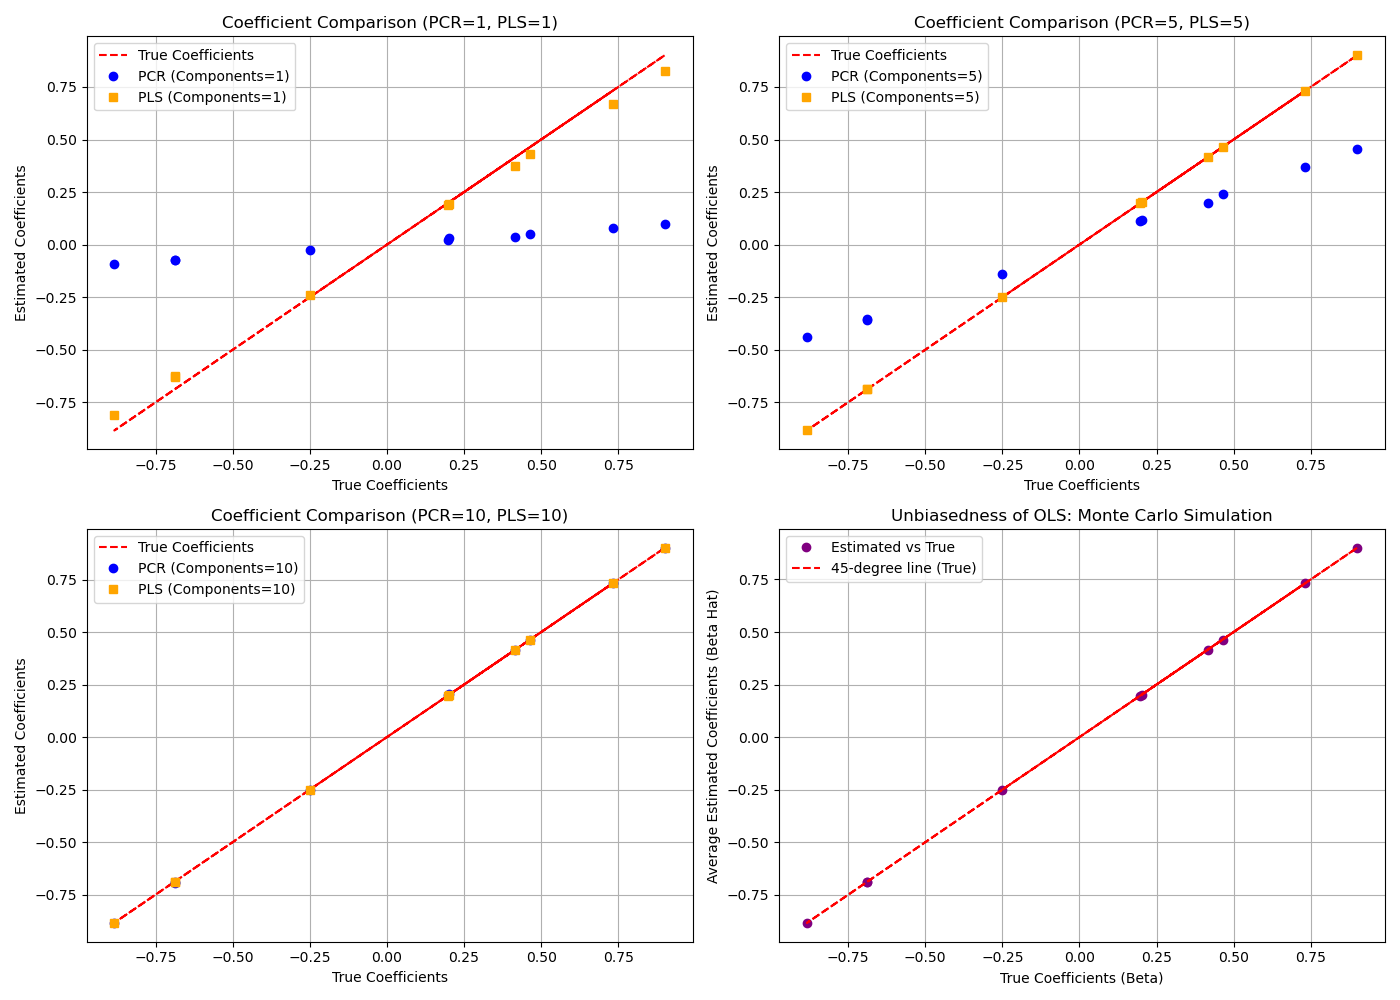
\includegraphics[width=0.9\textwidth]{First_plot.png}
    \caption{True vs Estimated coefficients: OLS, PCR and PLS}
    \label{fig:Classic_data_analysis}
\end{figure}

\begin{figure}[H]
    \centering
    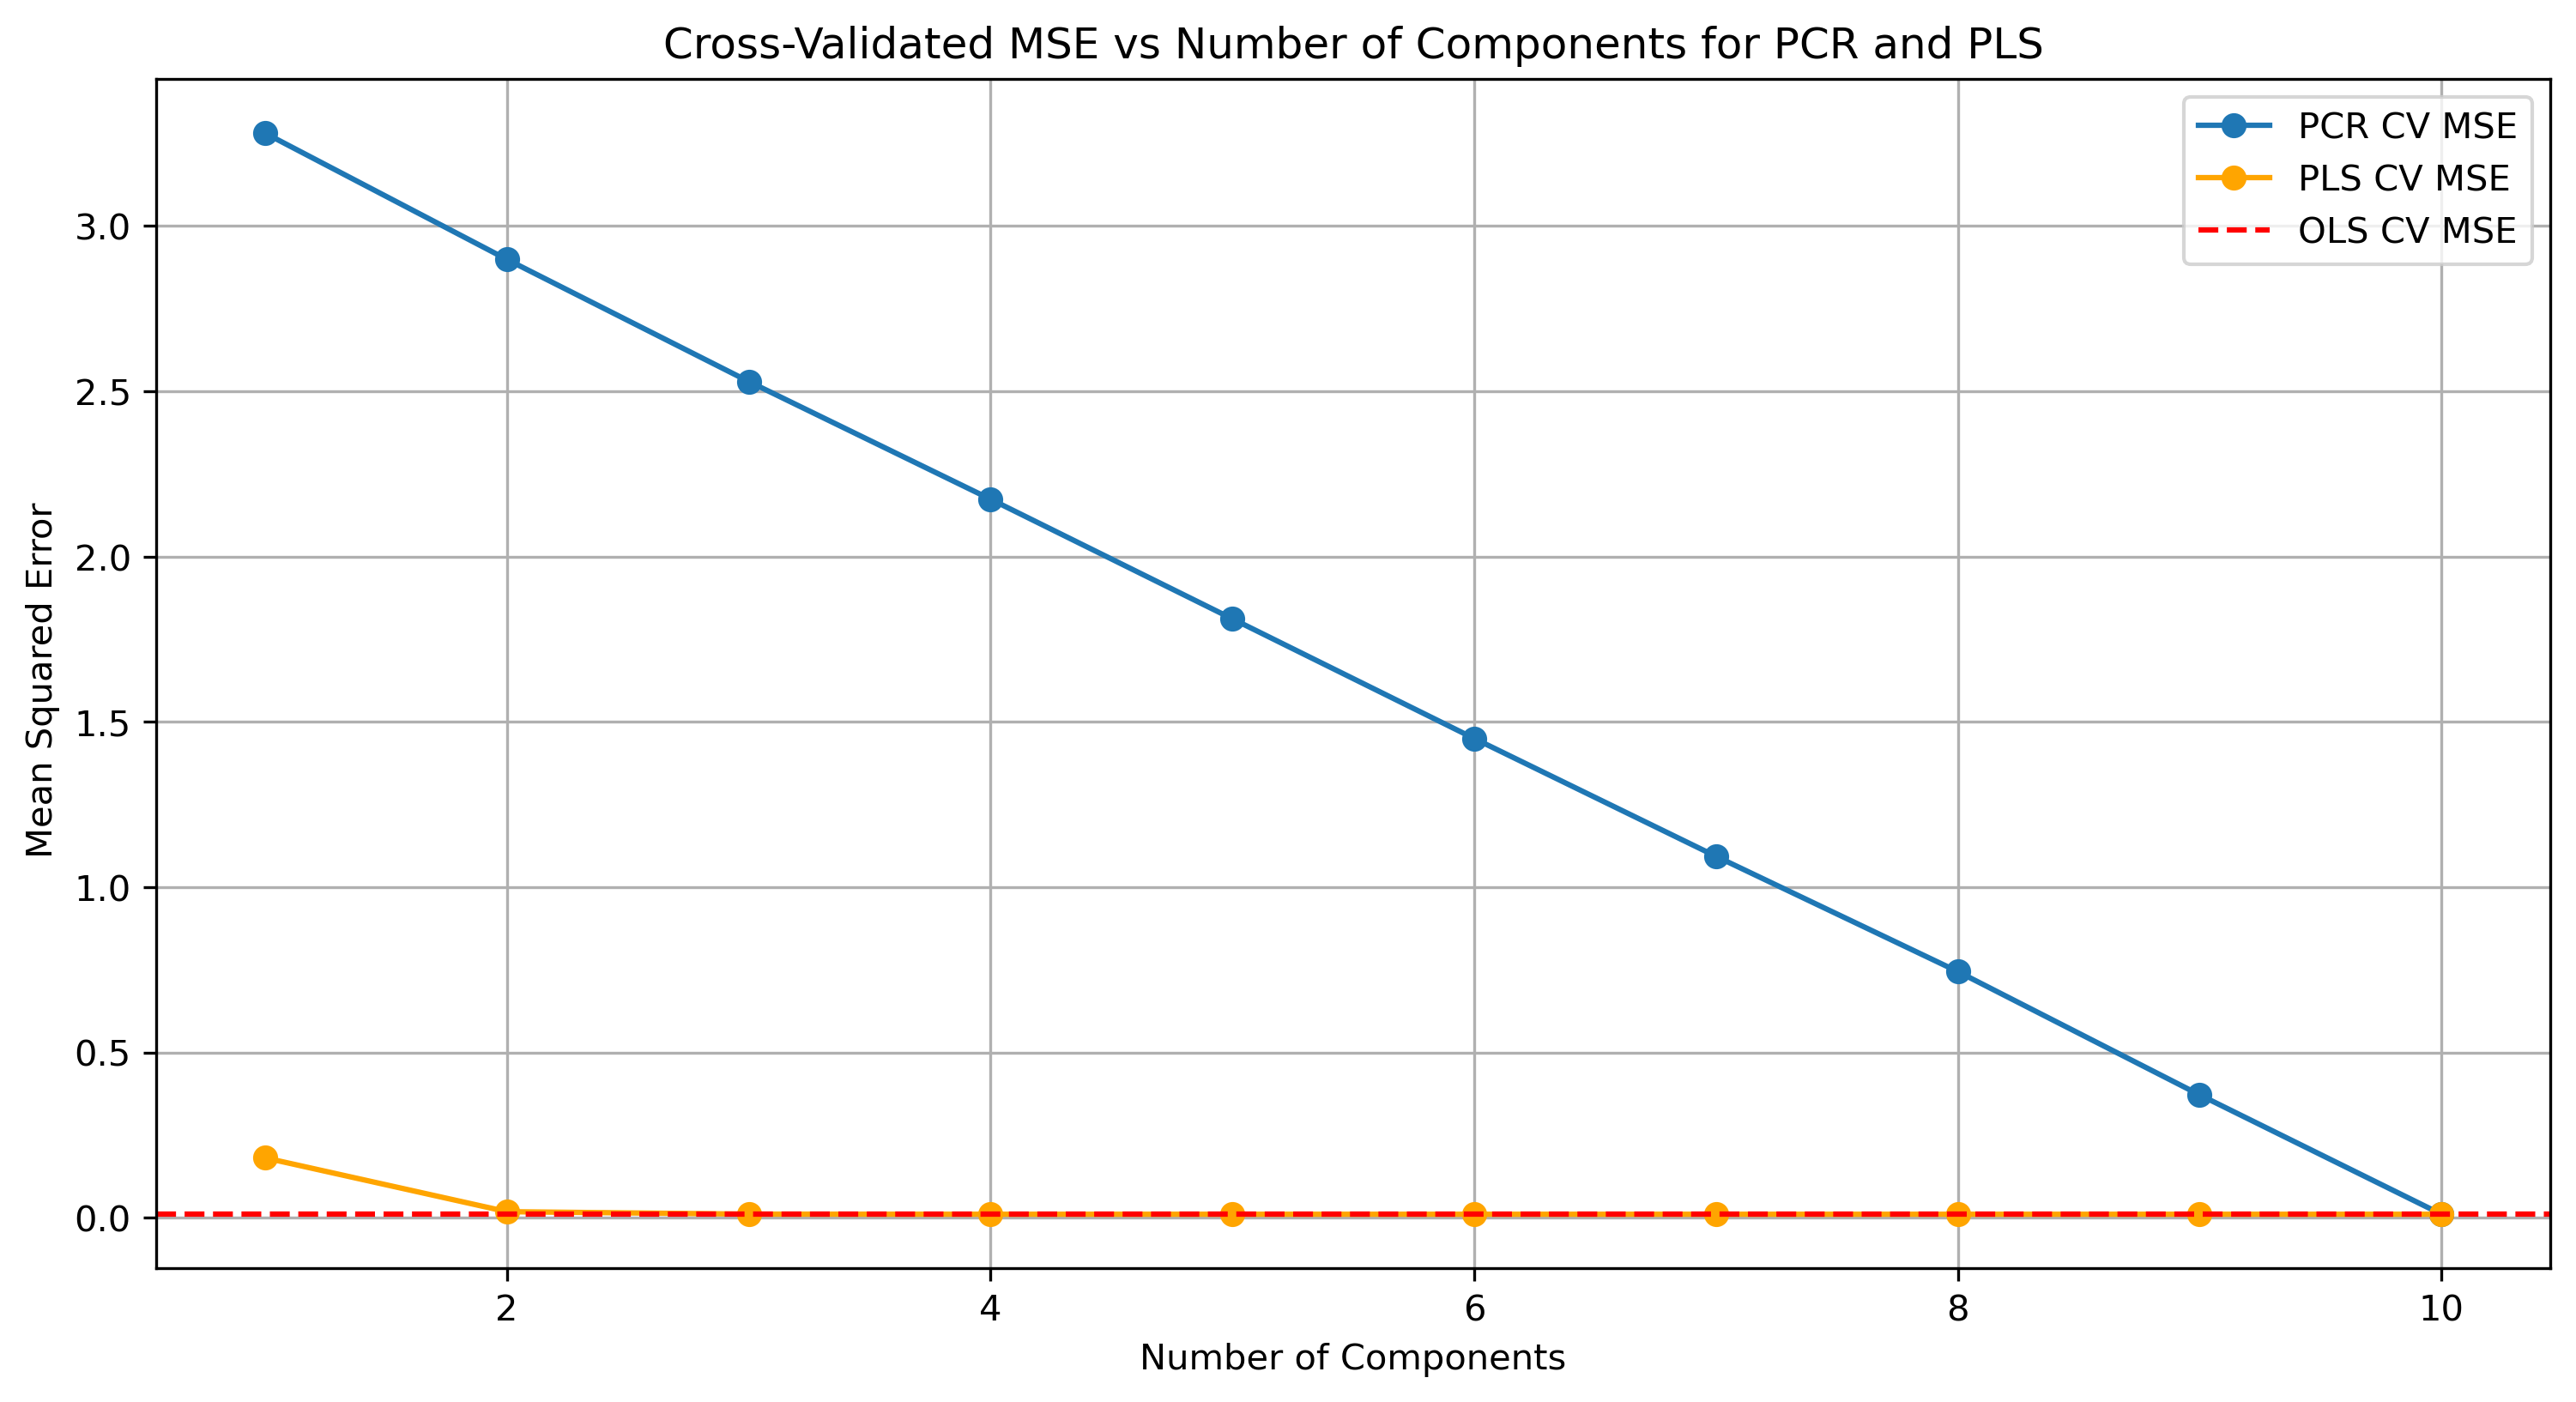
\includegraphics[width=0.9\textwidth]{Second_plot.png}
    \caption{CV MSE by components: OLS, PCR and PLS}
    \label{fig:Classic_data_analysis}
\end{figure}

\begin{figure}[H]
    \centering
    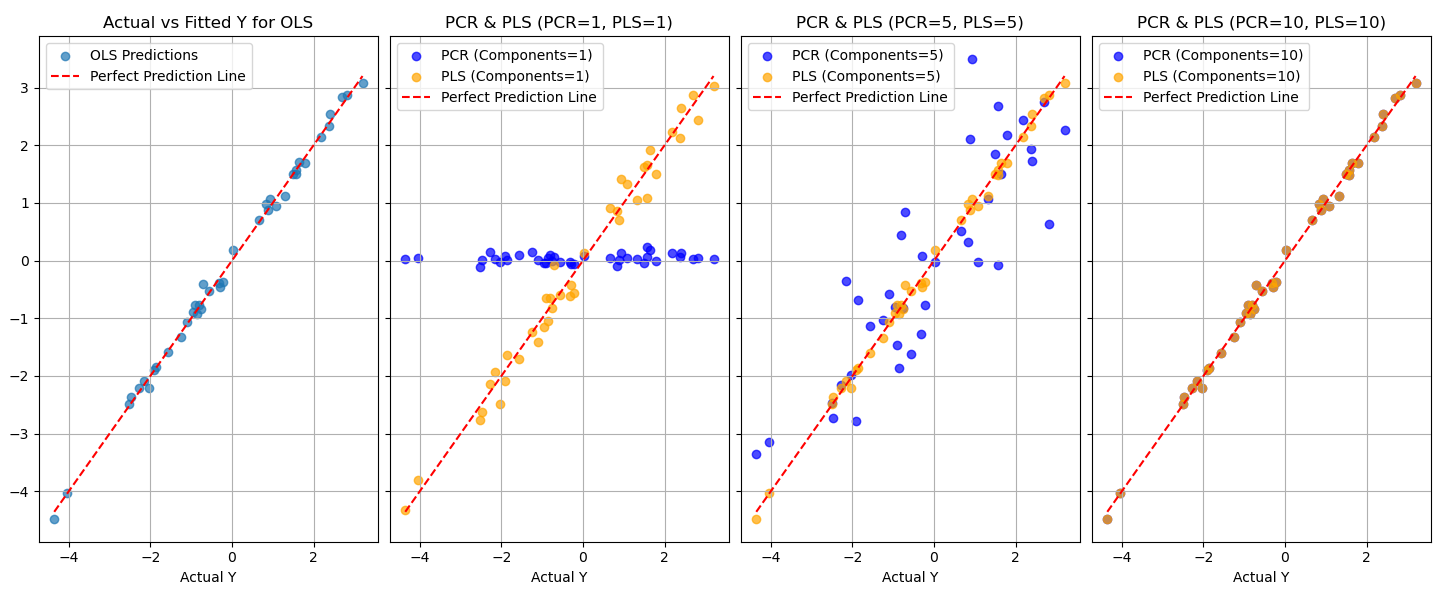
\includegraphics[width=0.9\textwidth]{Third_plot.png}
    \caption{Model fit: OLS, PCR and PLS}
    \label{fig:Classic_data_analysis}
\end{figure}

\begin{figure}[H]
    \centering
    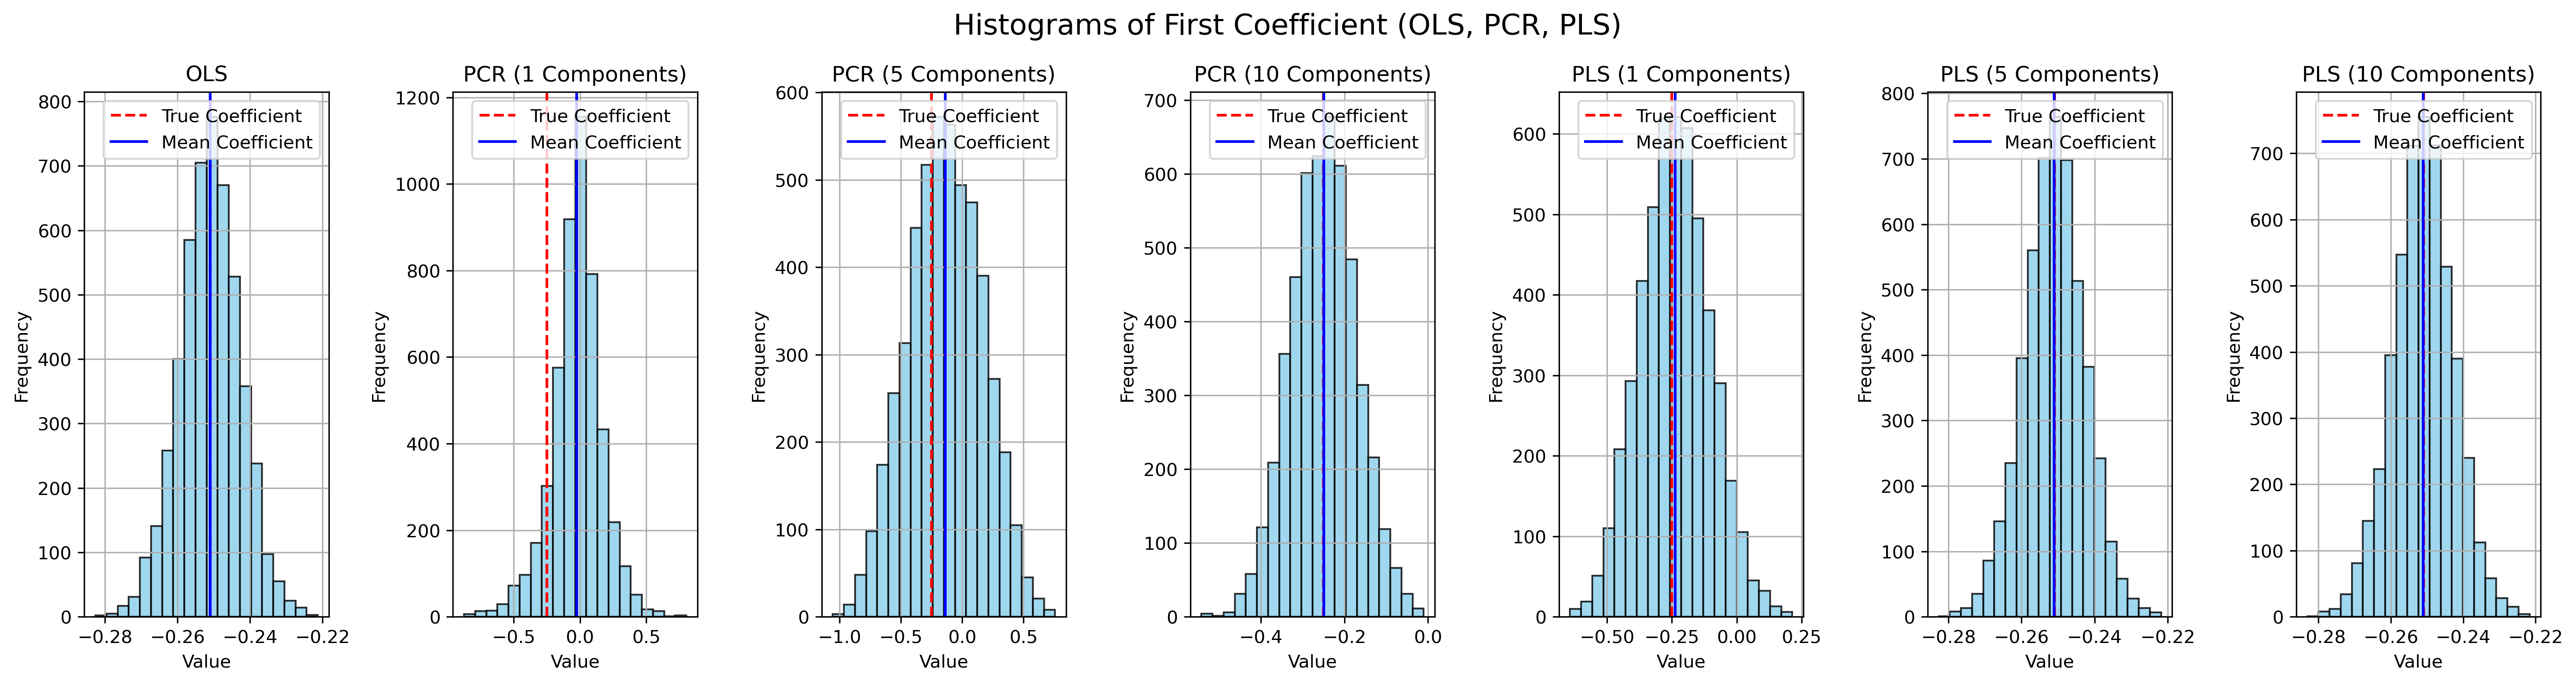
\includegraphics[width=0.9\textwidth]{Fourth_plot.png}
    \caption{Coefficient distribution: OLS, PCR and PLS}
    \label{fig:Classic_data_analysis}
\end{figure}

\subsection{Simulation Results: Moderate Multicollinearity Datase}

\begin{figure}[H]
    \centering
    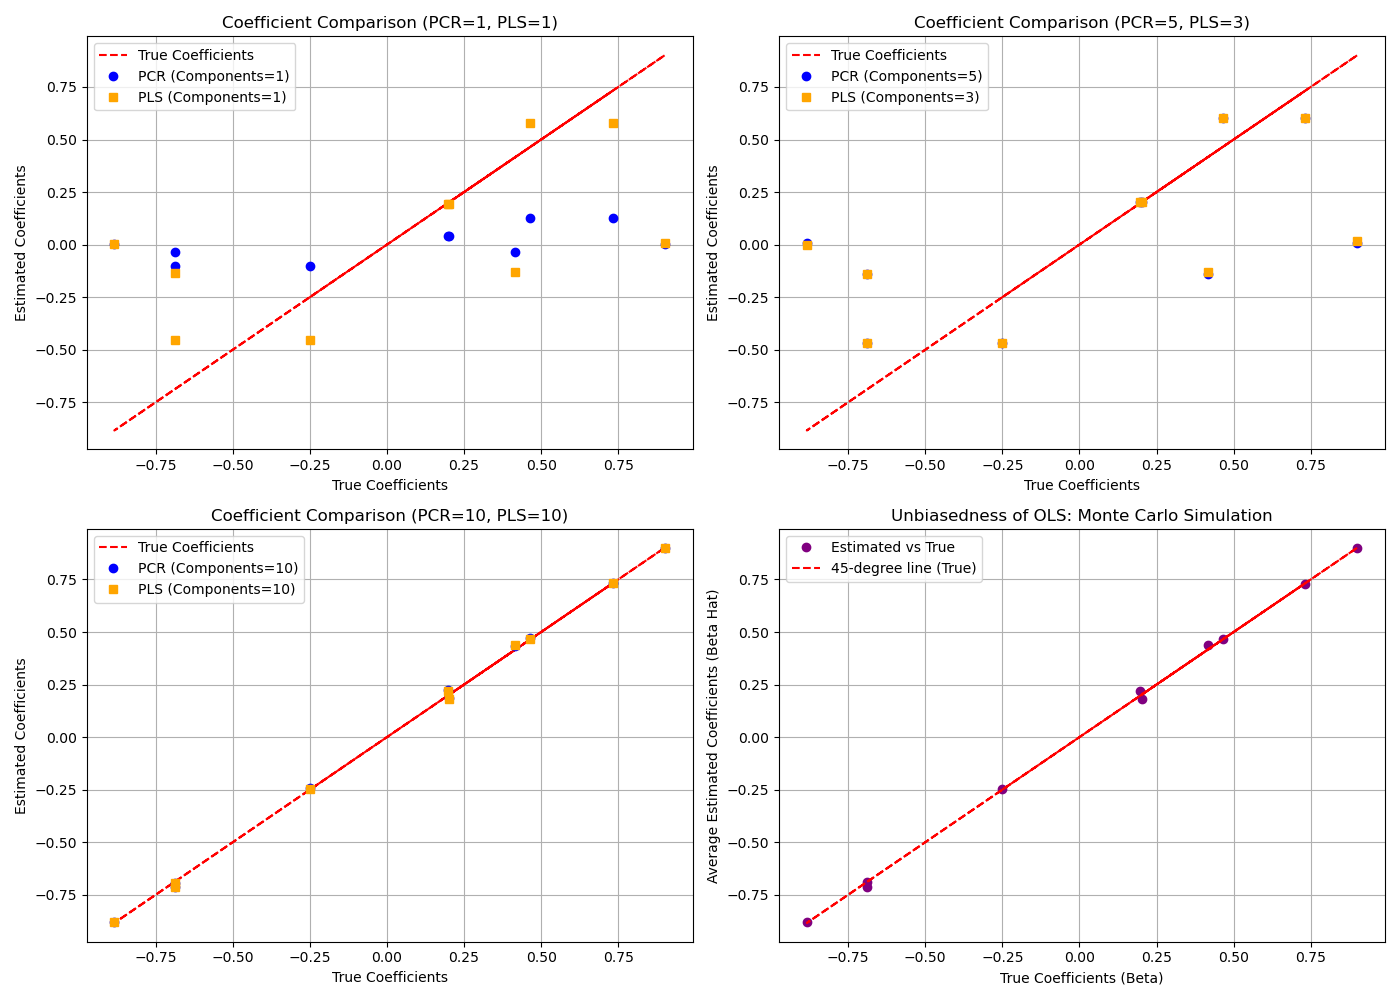
\includegraphics[width=0.9\textwidth]{First_plot_second_simulation.png}
    \caption{True vs Estimated coefficients: OLS, PCR and PLS}
    \label{fig:Moderate_multicollinear_data_analysis}
\end{figure}

\begin{figure}[H]
    \centering
    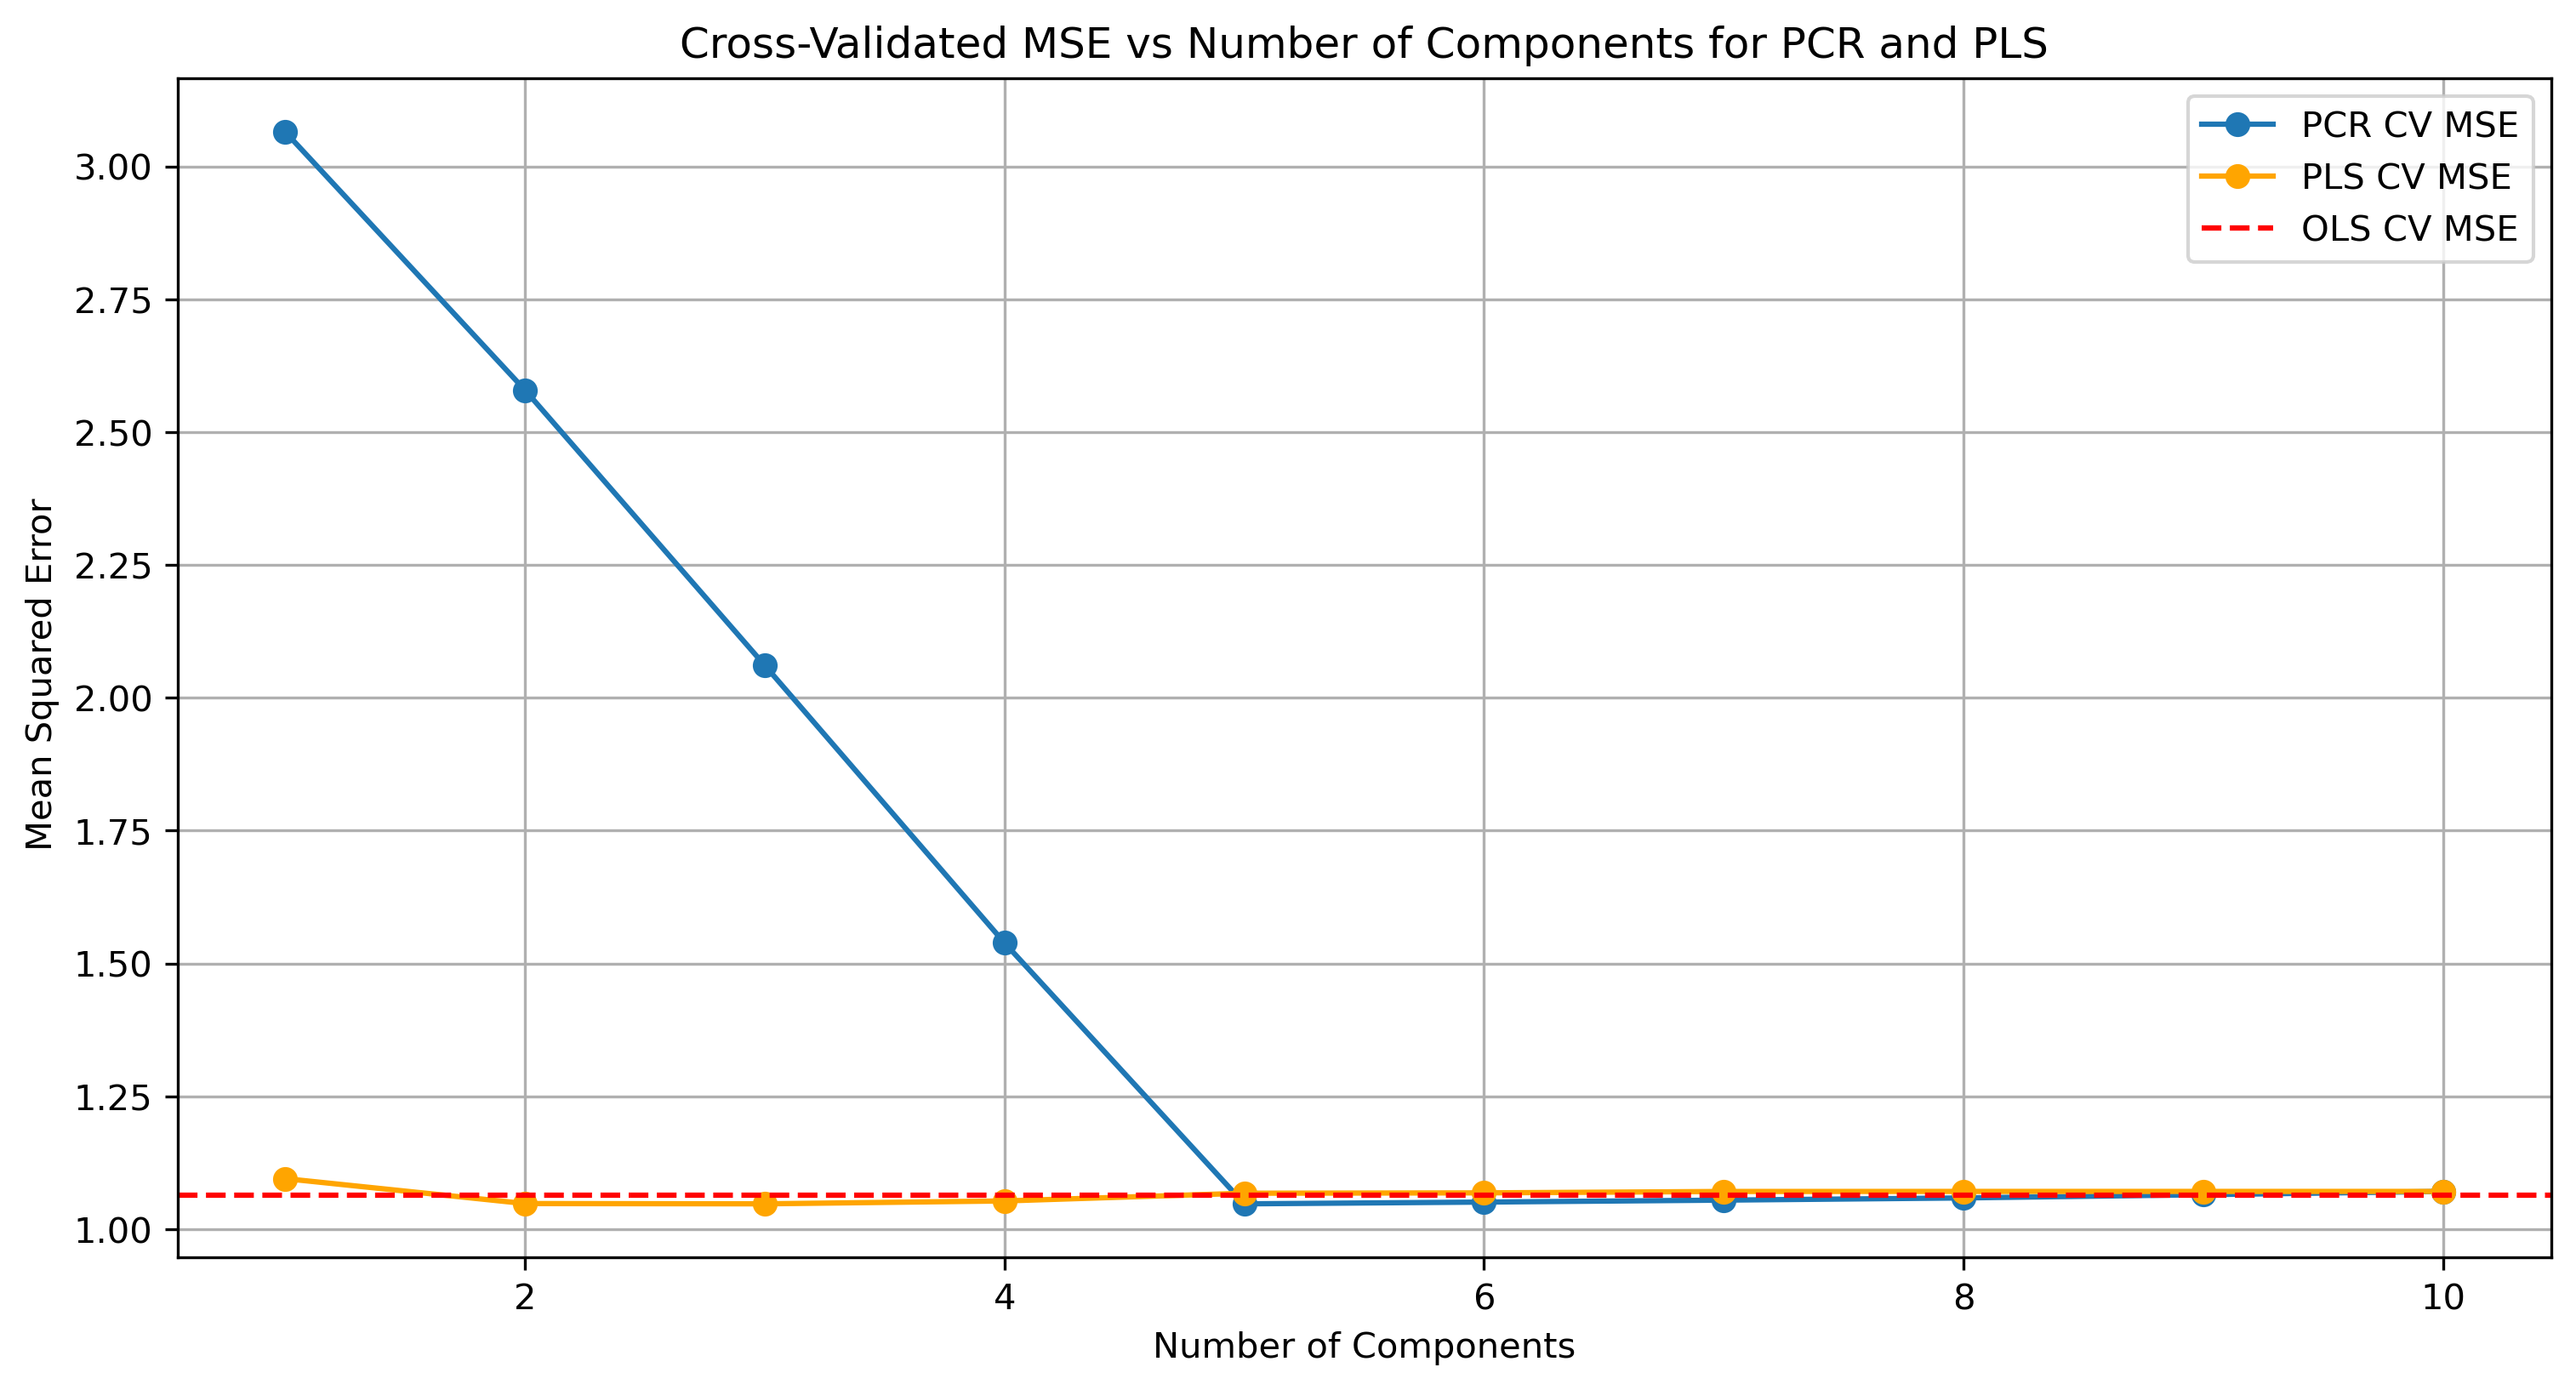
\includegraphics[width=0.9\textwidth]{Second_plot_second_simulation.png}
    \caption{CV MSE by components: OLS, PCR and PLS}
    \label{fig:Moderate_multicollinear_data_analysis}
\end{figure}

\begin{figure}[H]
    \centering
    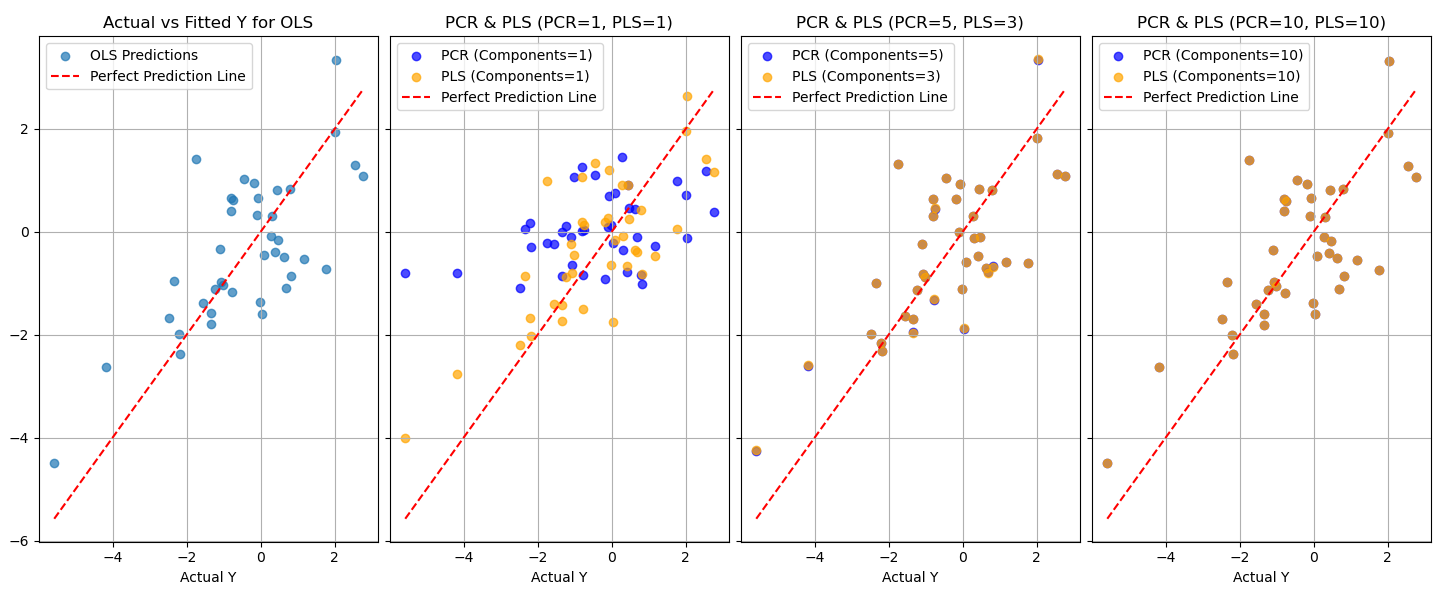
\includegraphics[width=0.9\textwidth]{Third_plot_second_simulation.png}
    \caption{Model fit: OLS, PCR and PLS}
    \label{fig:Moderate_multicollinear_data_analysis}
\end{figure}

\begin{figure}[H]
    \centering
    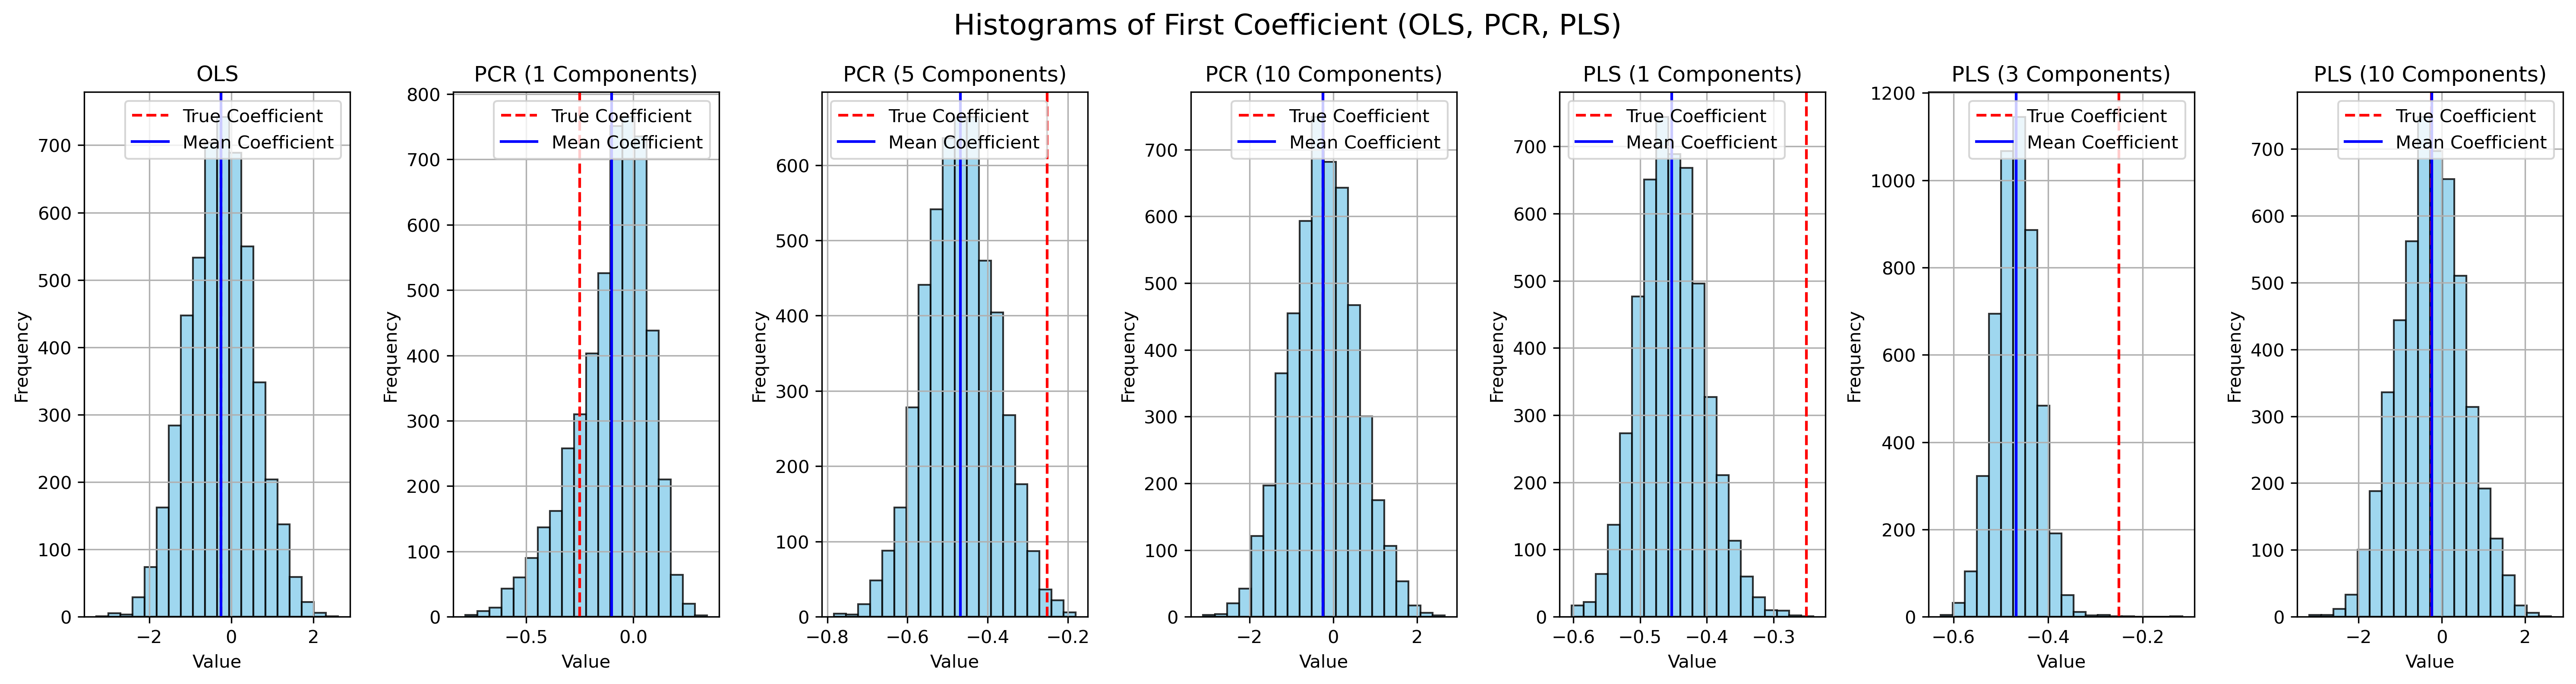
\includegraphics[width=0.9\textwidth]{Fourth_plot_second_simulation.png}
    \caption{Coefficient distribution: OLS, PCR and PLS}
    \label{fig:Moderate_multicollinear_data_analysis}
\end{figure}

\subsection{Simulation Results: Severe Multicollinearity with Low Observations}

\begin{figure}[H]
    \centering
    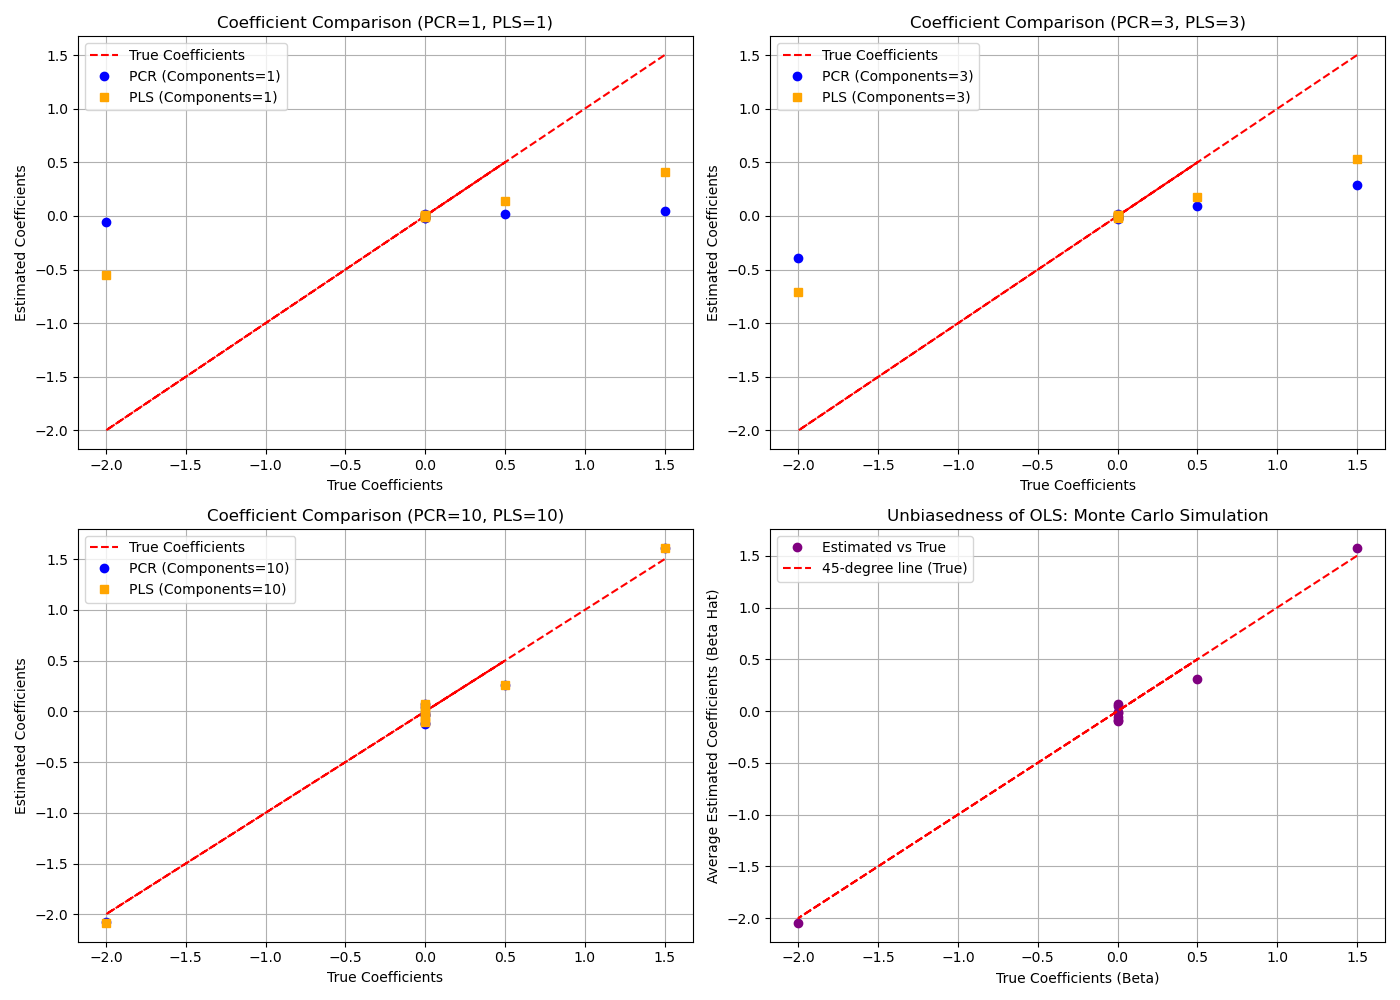
\includegraphics[width=0.9\textwidth]{First_plot_third_simulation.png}
    \caption{True vs Estimated coefficients: OLS, PCR and PLS}
    \label{fig:Severe_multicollinear_data_analysis}
\end{figure}

\begin{figure}[H]
    \centering
    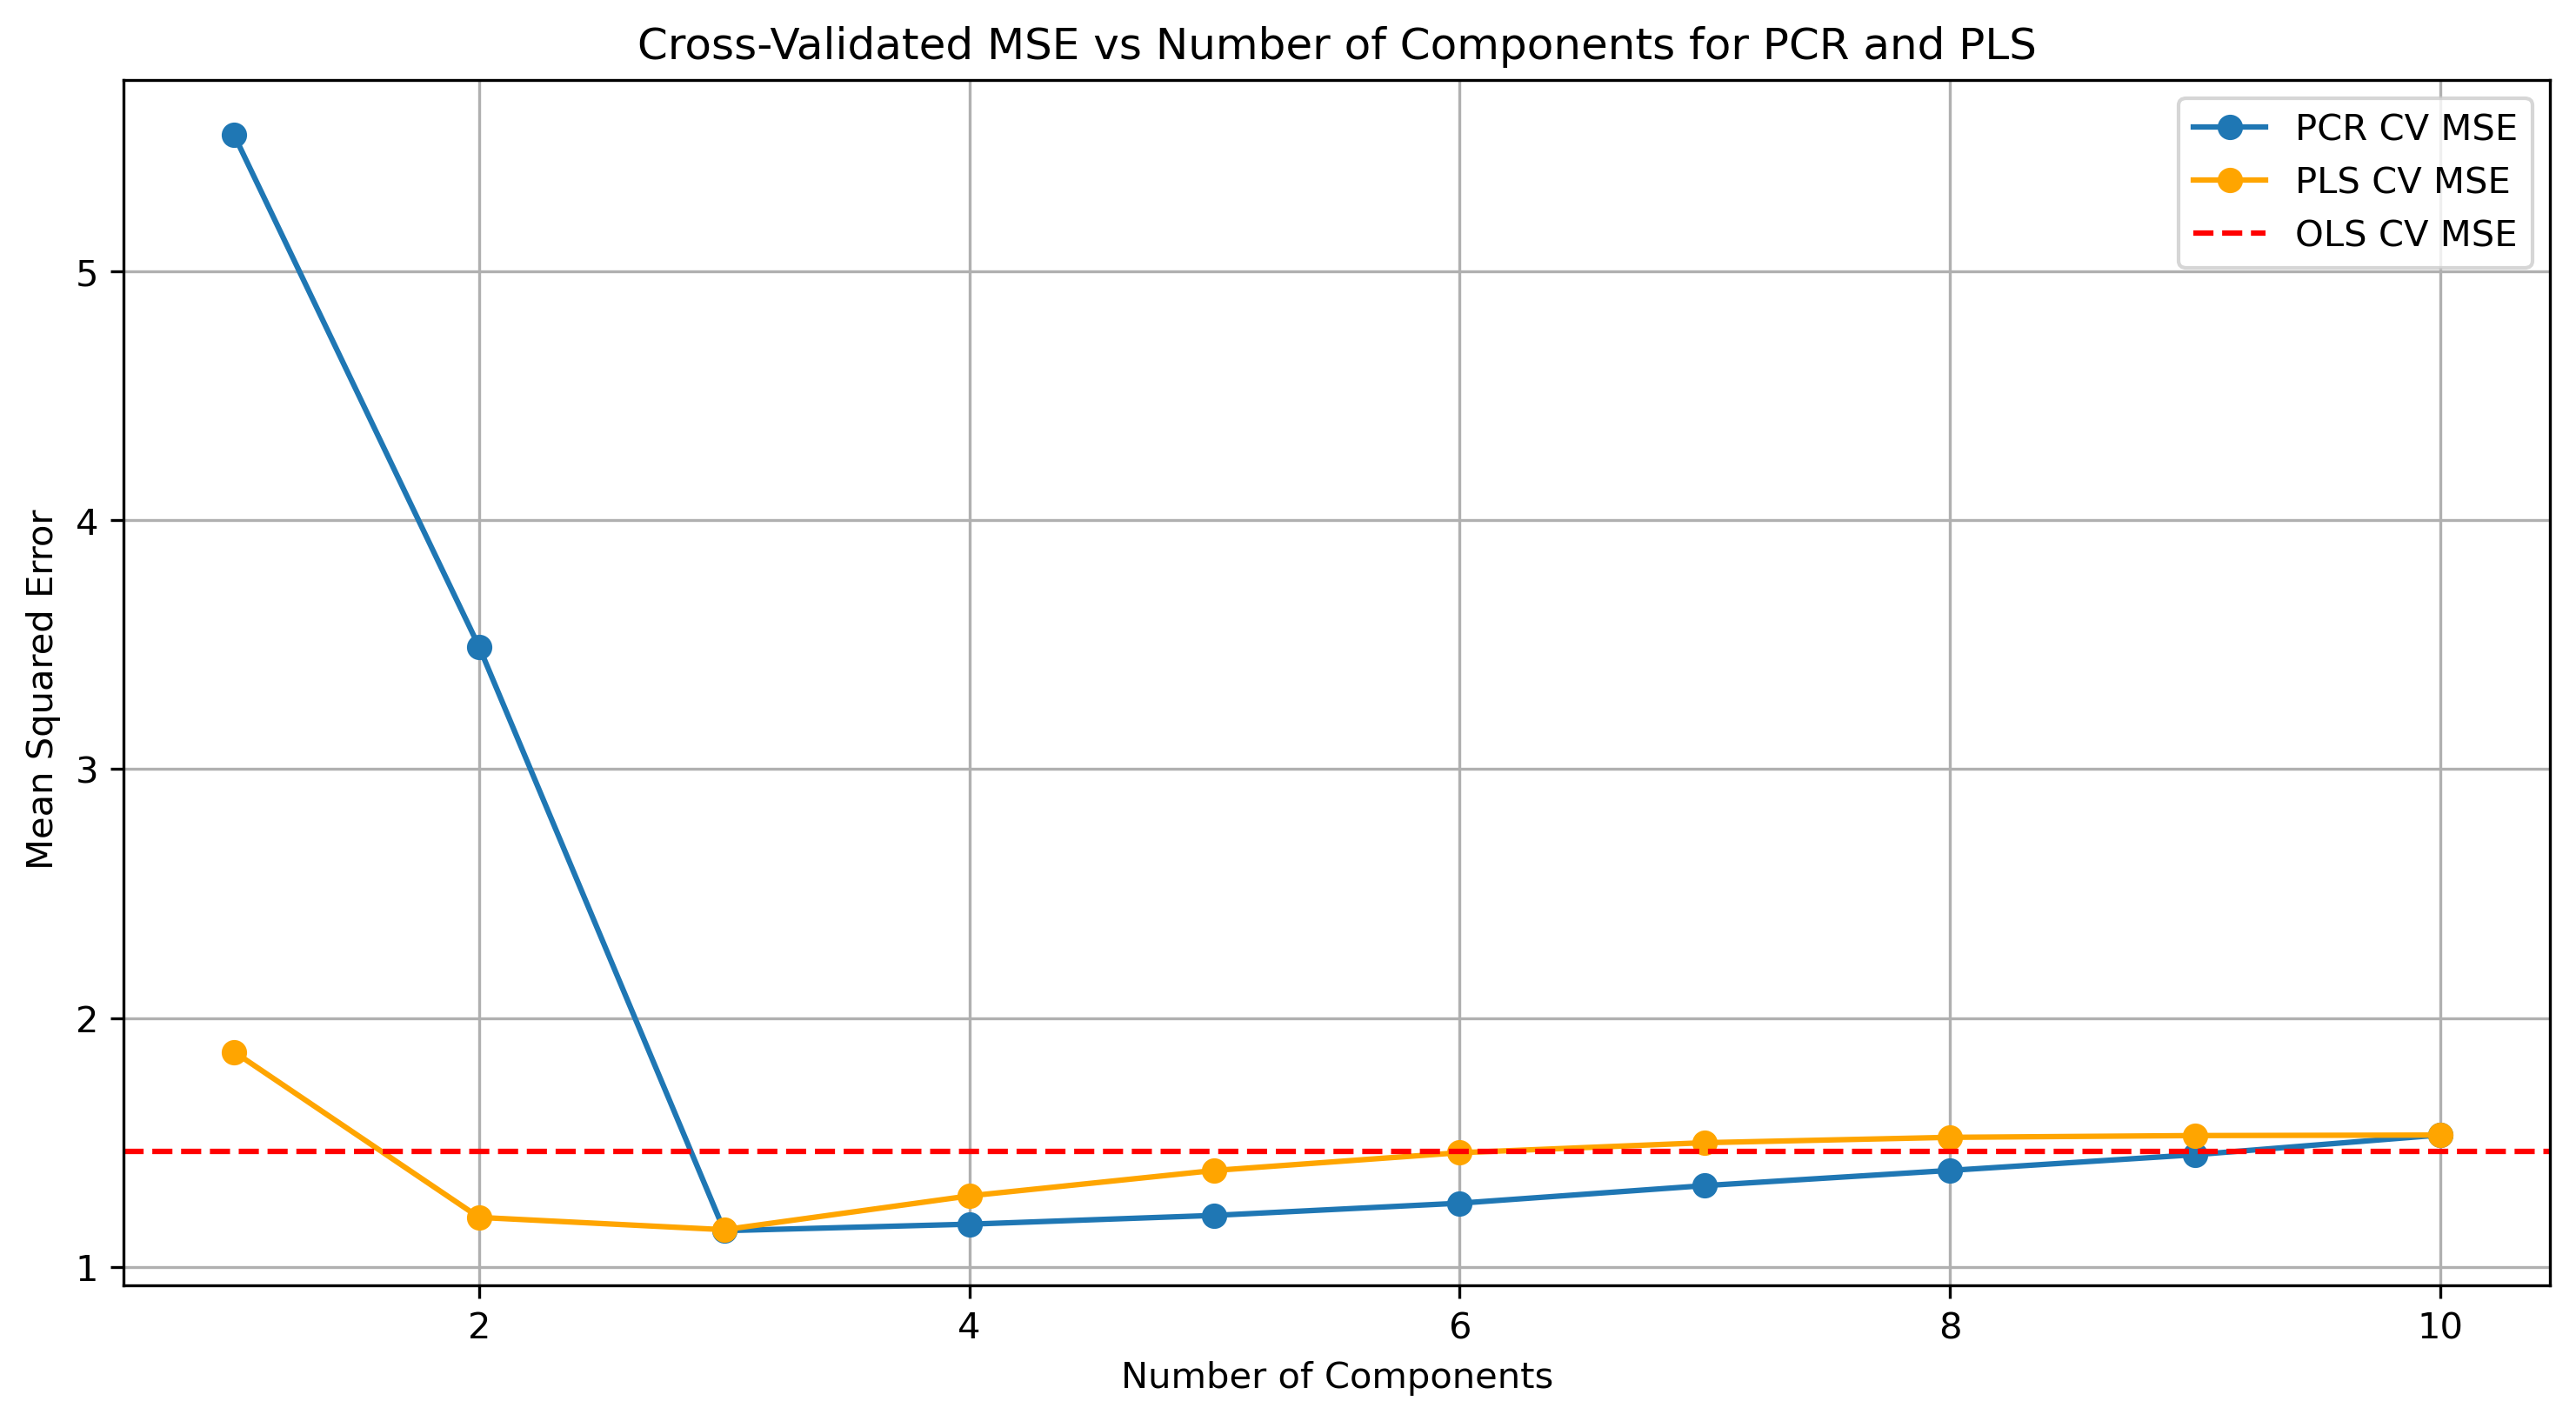
\includegraphics[width=0.9\textwidth]{Second_plot_third_simulation.png}
    \caption{CV MSE by components: OLS, PCR and PLS}
    \label{fig:Severe_multicollinear_data_analysis}
\end{figure}

\begin{figure}[H]
    \centering
    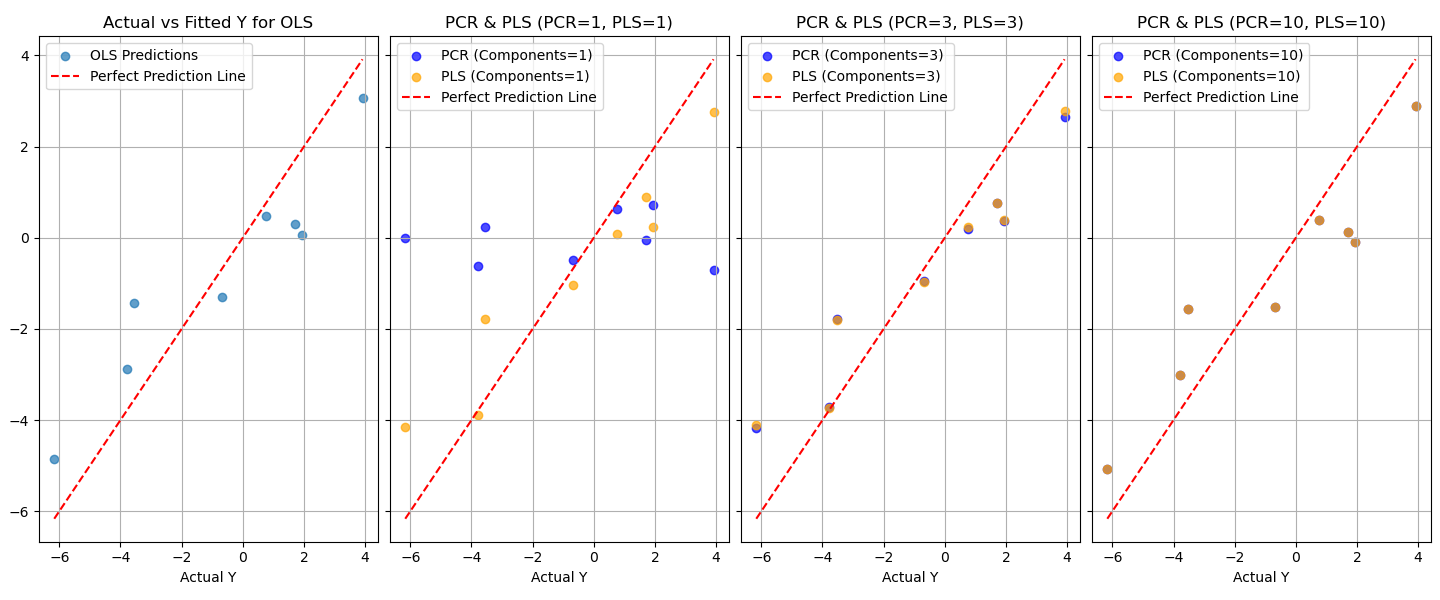
\includegraphics[width=0.9\textwidth]{Third_plot_third_simulation.png}
    \caption{Model fit: OLS, PCR and PLS}
    \label{fig:Severe_multicollinear_data_analysis}
\end{figure}

\begin{figure}[H]
    \centering
    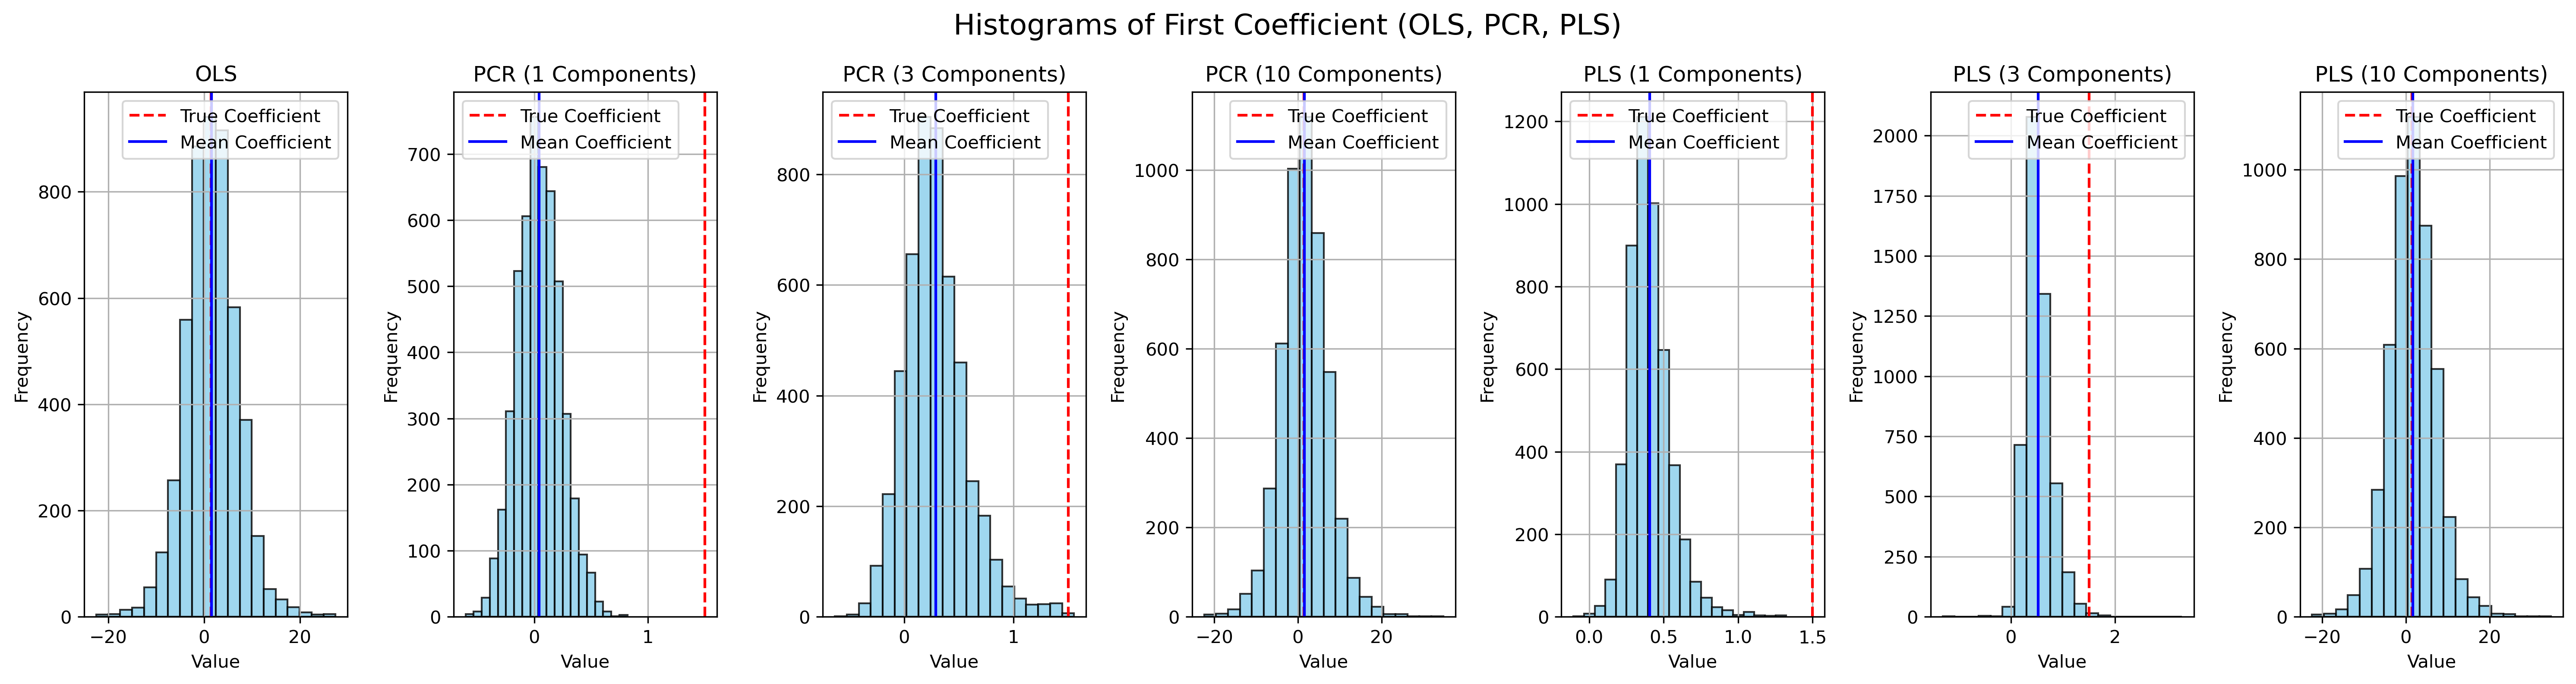
\includegraphics[width=0.9\textwidth]{Fourth_plot_third_simulation.png}
    \caption{Coefficient distribution: OLS, PCR and PLS}
    \label{fig:Severe_multicollinear_data_analysis}
\end{figure}

\subsection{Analysis of NIR Data: Corn Moisture Prediction Using PLS and PCR}

\begin{figure}[H]
    \centering
    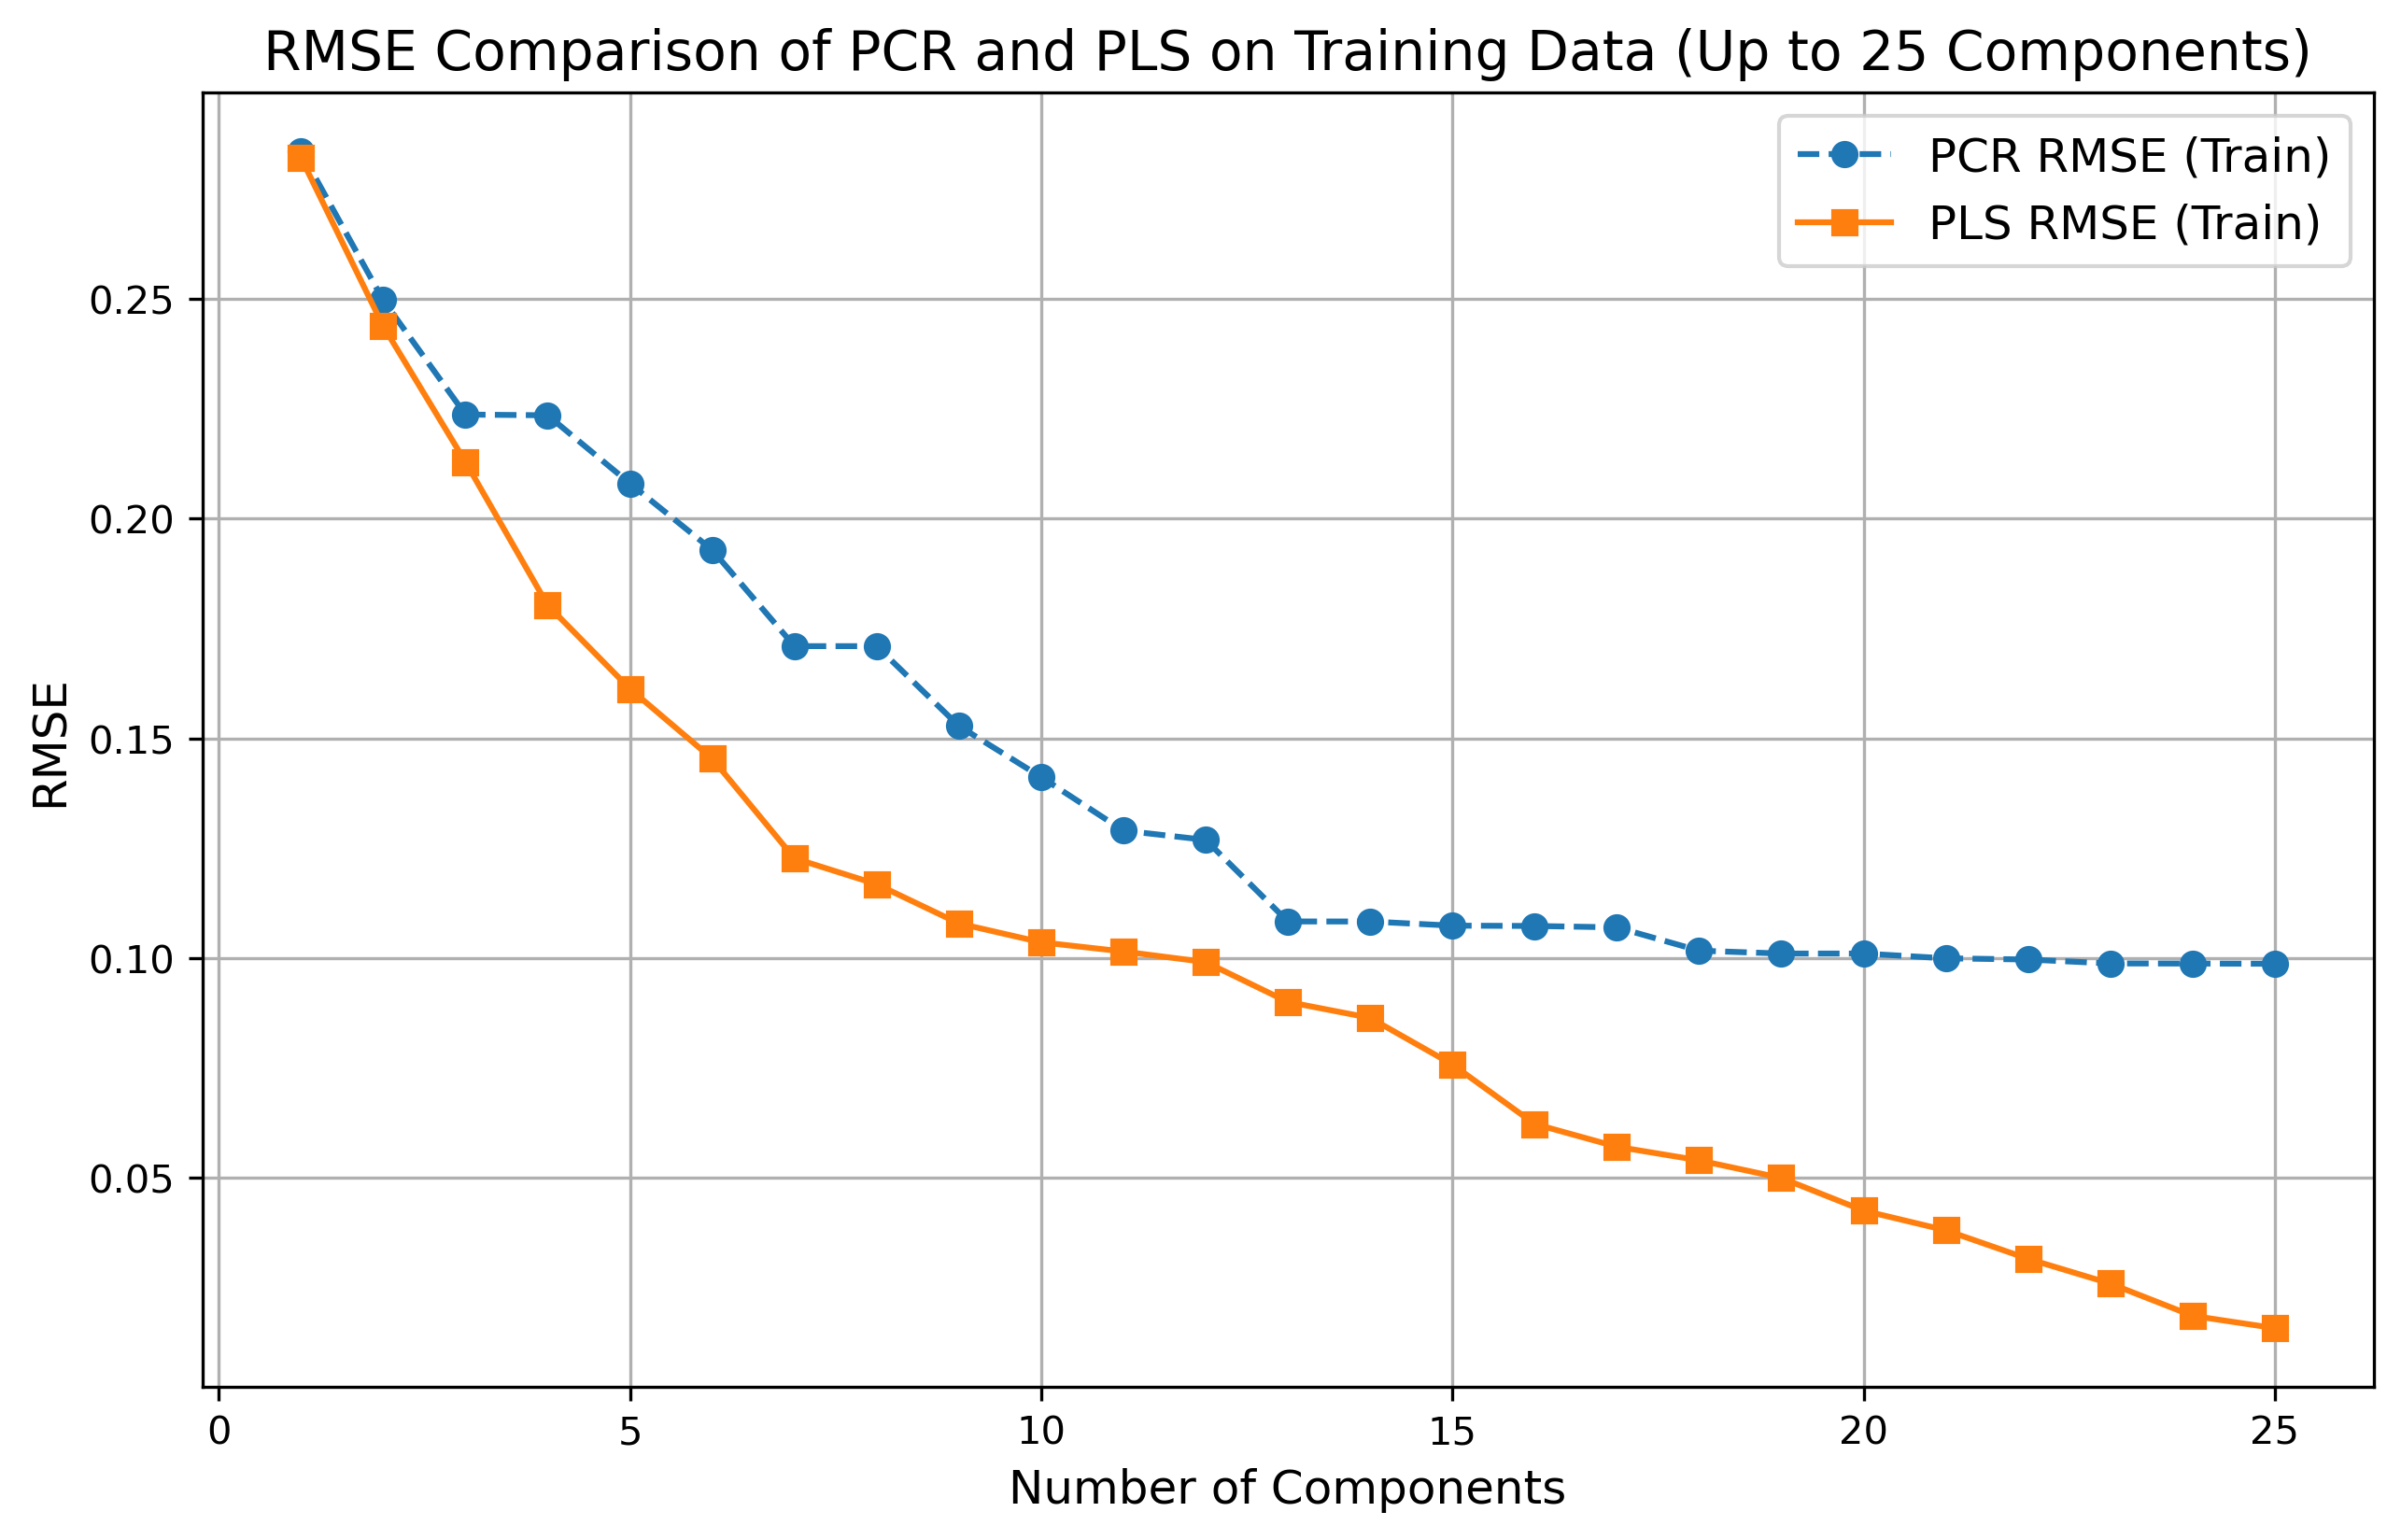
\includegraphics[width=0.9\textwidth]{NIR_second_plot.png}
    \caption{RMSE of PCR and PLS on training data}
    \label{fig:NIR_analysis}
\end{figure}

\begin{figure}[H]
    \centering
    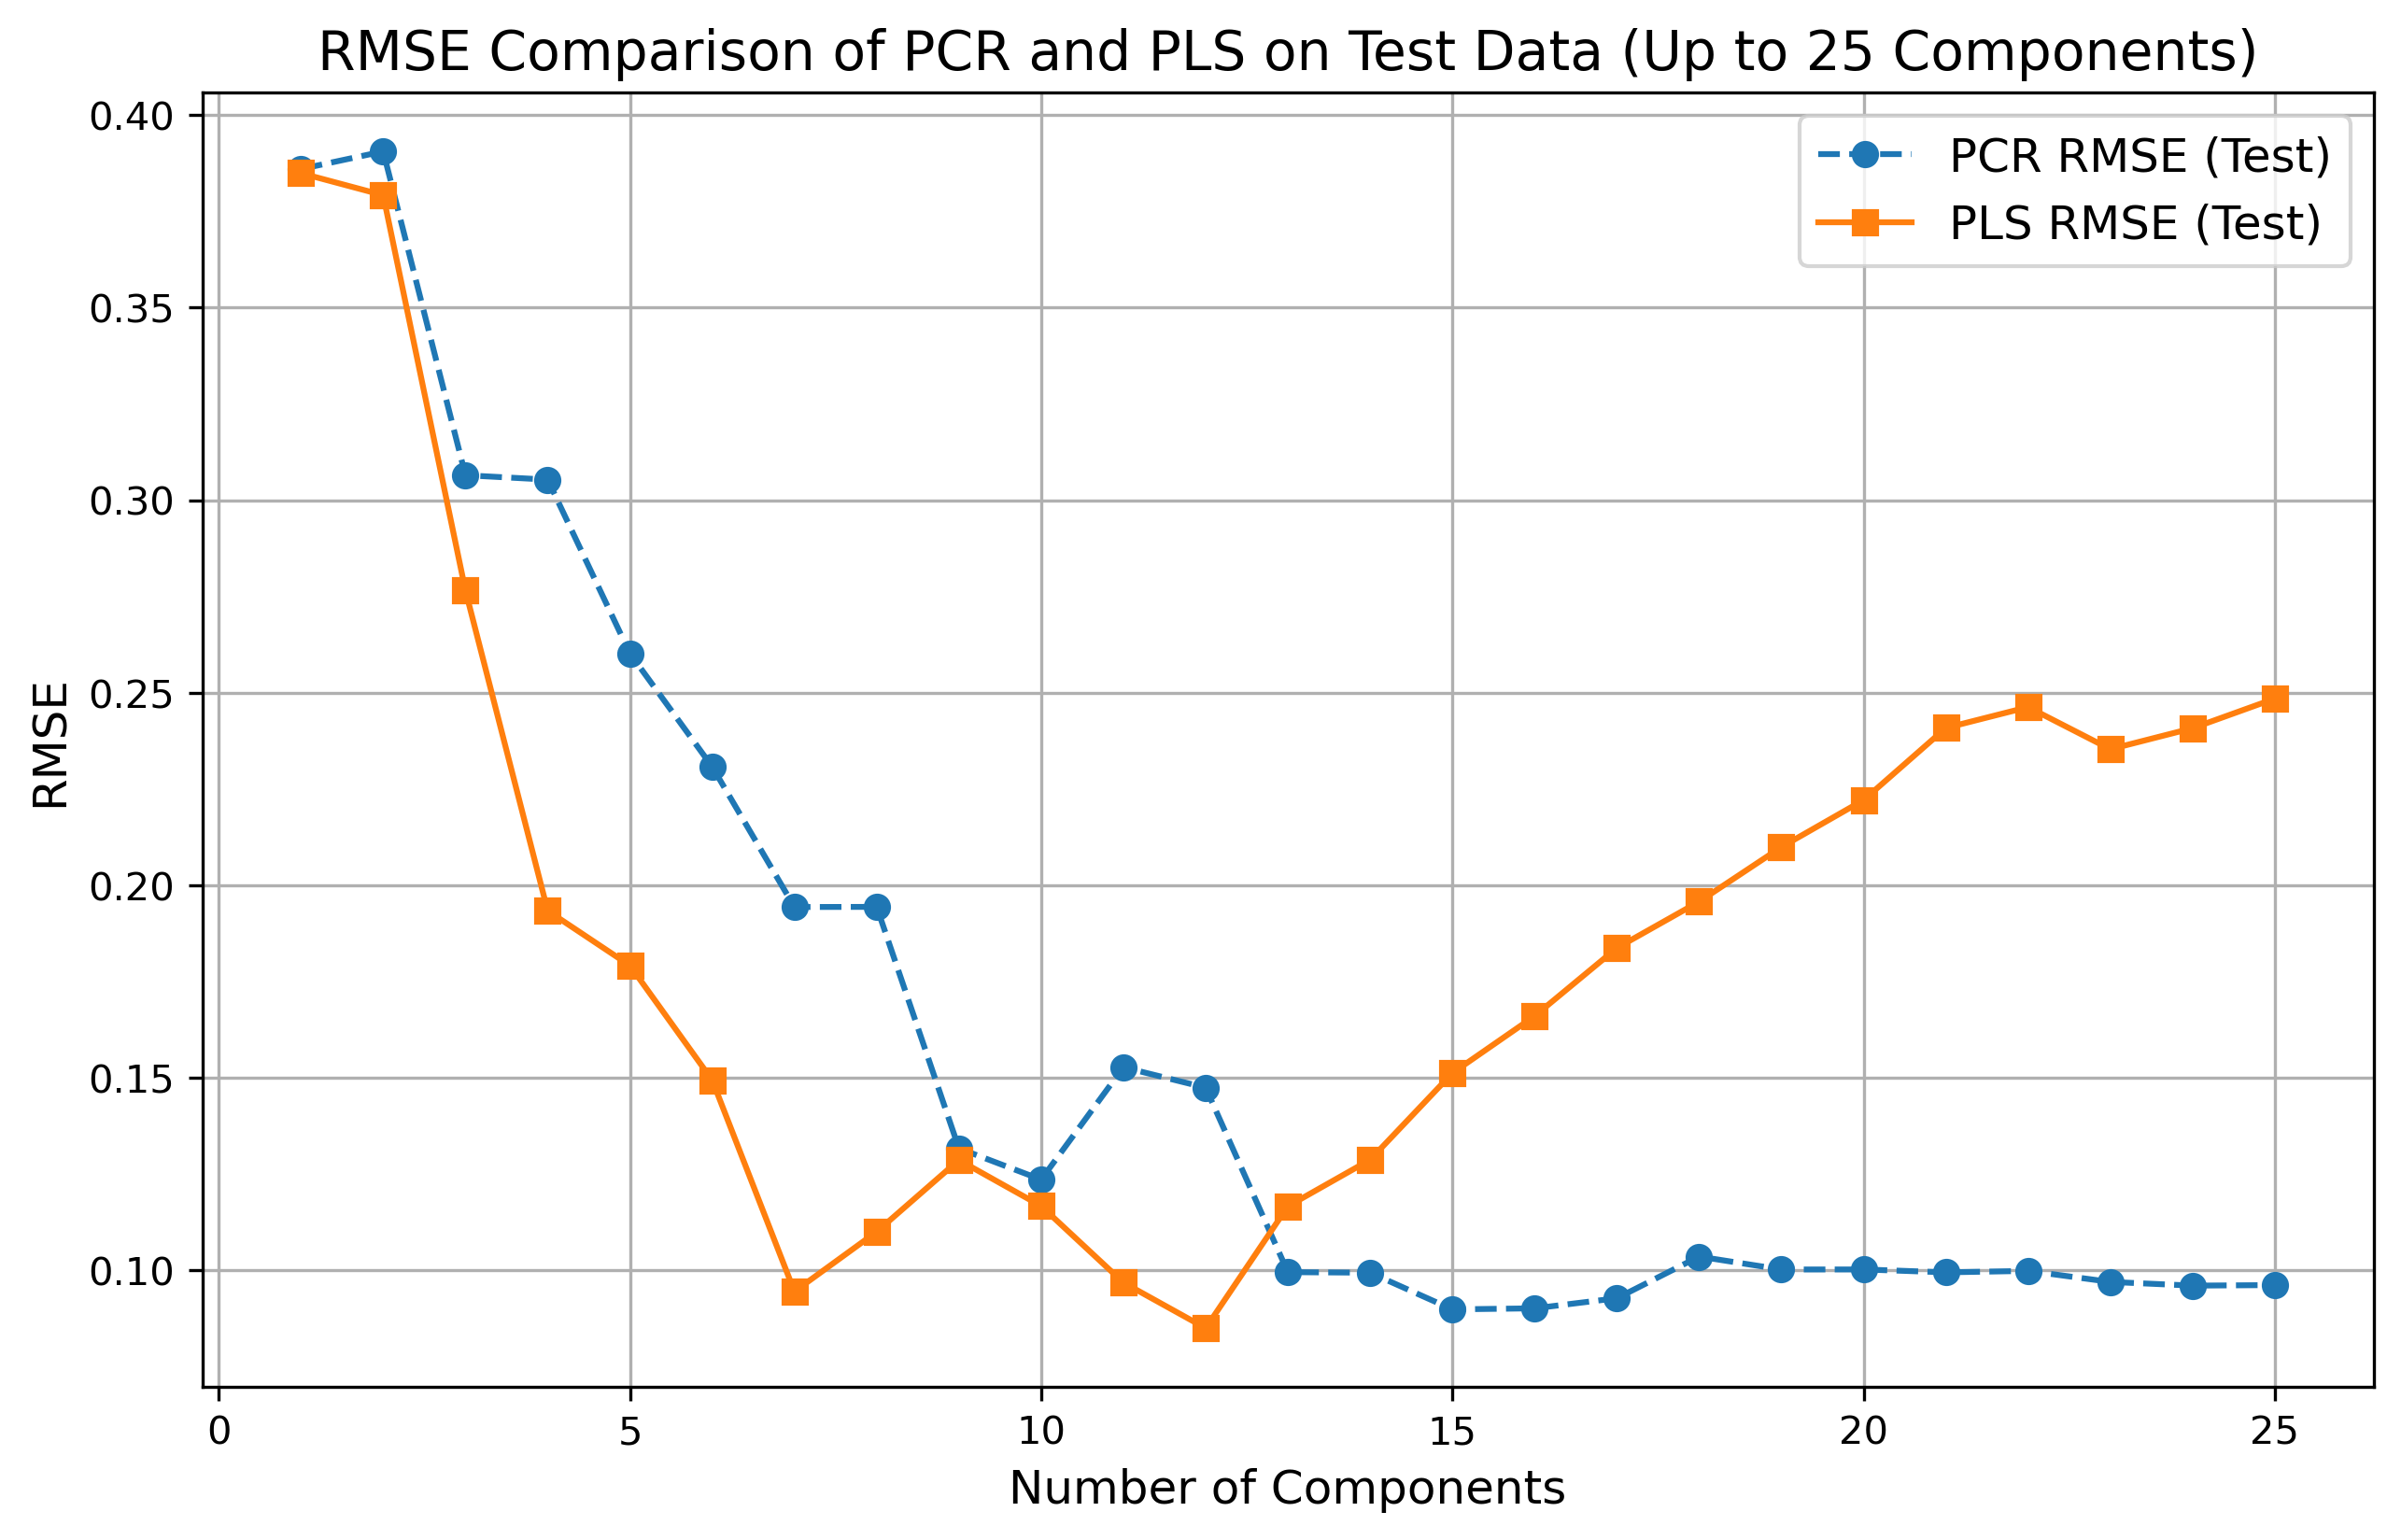
\includegraphics[width=0.9\textwidth]{NIR_third_plot.png}
    \caption{RMSE of PCR and PLS on test data}
    \label{fig:NIR_analysis}
\end{figure}

\begin{figure}[H]
    \centering
    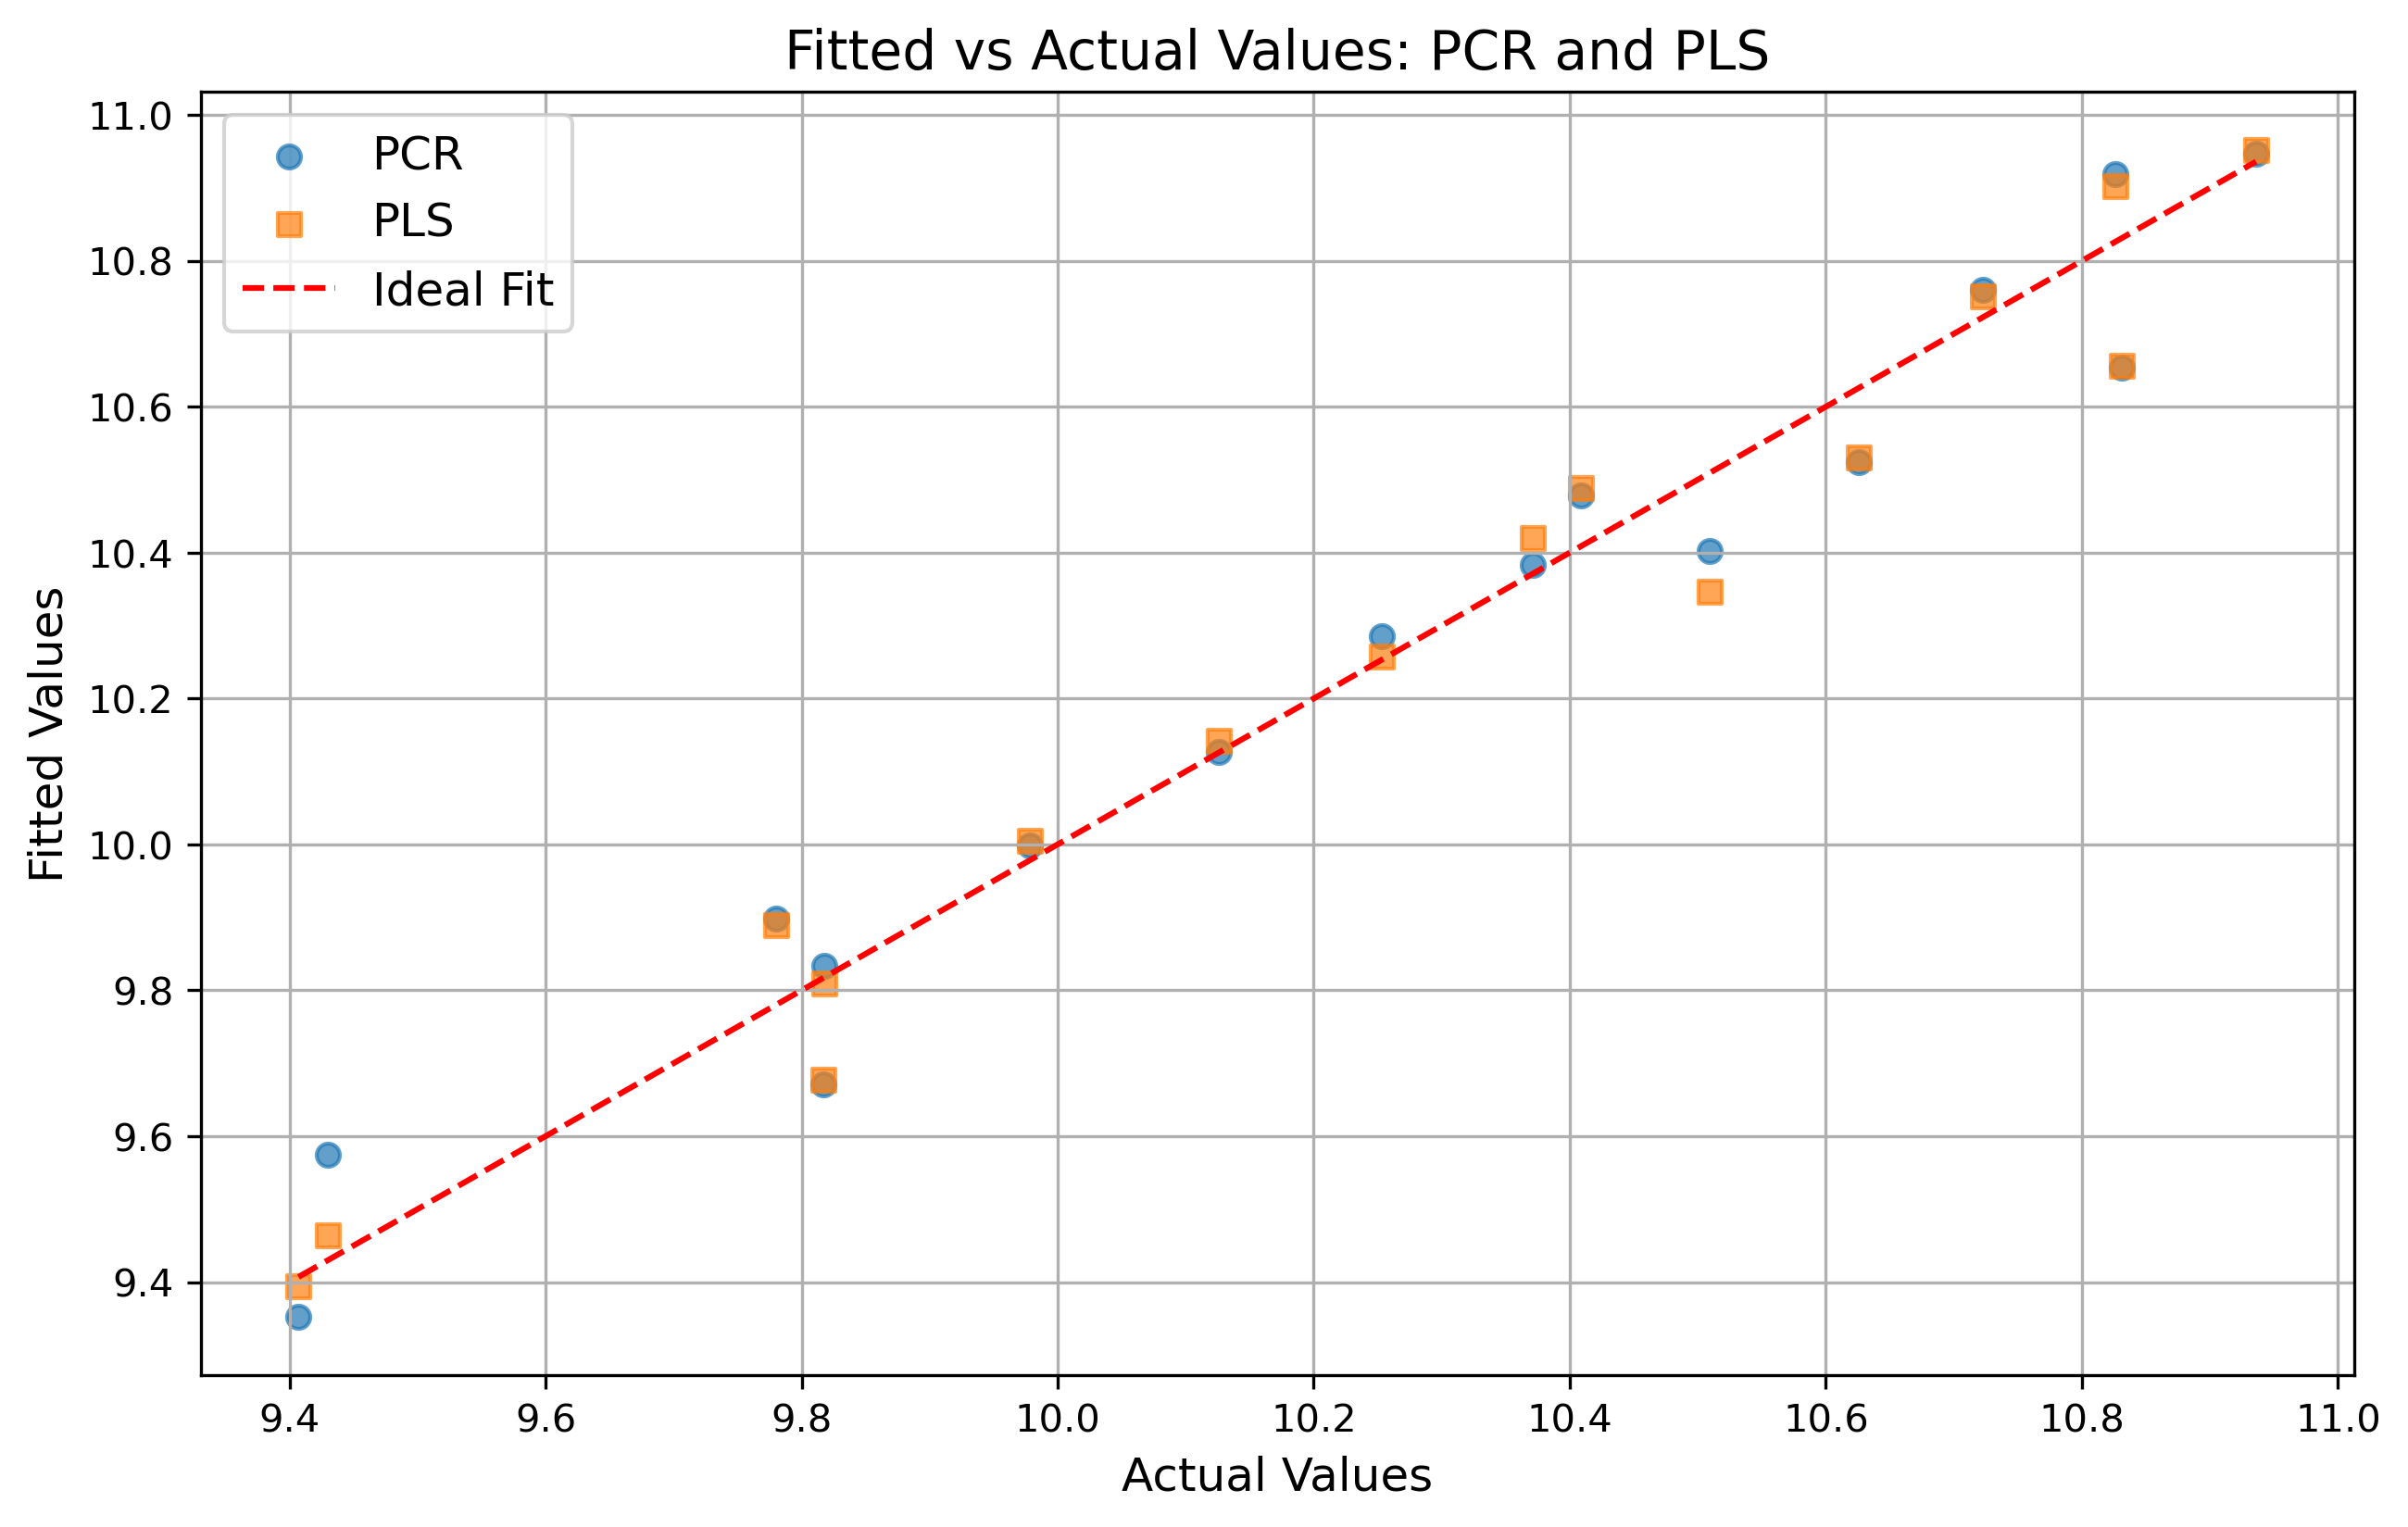
\includegraphics[width=0.9\textwidth]{NIR_fifth_plot.png}
    \caption{Actual and prediction models performance}
    \label{fig:NIR_analysis}
\end{figure}

\newpage
\subsection{Quantitative Results}

\begin{table}[h]
    \centering
    \begin{tabular}{|c|c|c|c|}
        \hline
        Methods & Optimal components & Avg CV MSE of prediction & Dataset: Multicollinearity level \\
        \hline
        OLS & NA & 0.0106 & \multirow{3}{*}{No multicollinearity} \\
        PCR & 10 & 0.0106 &  \\
        PLS & 10 & 0.0106 &  \\
        \hline
        OLS & NA & 1.0642 & \multirow{3}{*}{Moderate} \\        
        PCR & 5 & 1.0477 &  \\
        PLS & 3 & 1.0477 &  \\
        \hline
        OLS & NA & 1.4639 & \multirow{3}{*}{Severe} \\
        PCR & 3 & 1.1452 &  \\
        PLS & 3 & 1.1492 &  \\ 
        \hline  
        OLS & NA & NA & \multirow{3}{*}{NIR spectroscopy data} \\
        PCR & 15 & 0.0898 &  \\
        PLS & 12 & 0.0849 &  \\ 
        \hline
    \end{tabular}
    \caption{Prediction accuracy and optimal components across different multicollinearity levels}
    \label{tab:multicollinearity_comparison}
\end{table}


\begin{table}[h]
    \centering
    \begin{tabular}{|c|c|c|c|c|}
        \hline
        Methods & Avg MSE of regression coefficients &  $\text{Bias}^2$ & Variance & Dataset: Multicollinearity level \\
        \hline
        OLS & 0.0001 & 0.0 & 0.0001 & \multirow{3}{*}{No multicollinearity} \\
        PCR & 0.0063 & 0.0 & 0.0063 &  \\
        PLS & 0.0001 & 0.0 & 0.0001 &  \\
        \hline
        OLS & 0.6598 & 0.0002 & 0.6596 & \multirow{3}{*}{Moderate} \\        
        PCR & 0.2414 & 0.2334 & 0.0080 &  \\
        PLS & 0.2305 & 0.2285 & 0.0020 &  \\
        \hline
        OLS & 12.7383 & 0.0072 & 12.7310 & \multirow{3}{*}{Severe} \\
        PCR & 0.5993 & 0.4221 & 0.1772 &  \\
        PLS & 0.4118 & 0.2719 & 0.1400 &  \\ 
        \hline
    \end{tabular}
    \caption{MSE coefficient decomposition across different different multicollinearity levels}
    \label{tab:Stability_analysis}
\end{table}
\newpage

\renewcommand\refname {\section {Bibliography}}

\begin{thebibliography}{99}

\bibitem{Hastie2009}
Hastie, Trevor, Tibshirani, Robert, and Friedman, Jerome. (2009). \textit{The Elements of Statistical Learning: Data Mining, Inference, and Prediction}. Springer. DOI: \href{https://doi.org/10.1007/978-0-387-84858-7}{10.1007/978-0-387-84858-7}

\bibitem{James2021}
James, Gareth, Witten, Daniela, Hastie, Trevor, and Tibshirani, Robert. (2021). \textit{An Introduction to Statistical Learning: with Applications in R}. Springer. DOI: \href{https://doi.org/10.1007/978-1-0716-1418-1}{10.1007/978-1-0716-1418-1}

\bibitem{Brunton2019}
Brunton, Steven L., and Kutz, J. Nathan. (2019). \textit{Data-Driven Science and Engineering: Machine Learning, Dynamical Systems, and Control}. Cambridge University Press. DOI: \href{https://doi.org/10.1017/9781108380690}{10.1017/9781108380690}

\bibitem{Johnstone2009}
Johnstone, Iain M., and Lu, Arthur Yu. (2009). On consistency and sparsity for principal components analysis in high dimensions. \textit{Journal of the American Statistical Association}, 104(486), 682–693. DOI: \href{https://doi.org/10.1198/jasa.2009.0121}{10.1198/jasa.2009.0121}

\bibitem{Greenberg1975}
Greenberg, Edward. (1975). Minimum variance properties of principal component regression. \textit{Journal of the American Statistical Association}, 70(349), 194–197. DOI: \href{https://doi.org/10.1080/01621459.1975.10480287}{10.1080/01621459.1975.10480287}

\bibitem{Agarwal2021}
Agarwal, Anish, Shah, Devavrat, Shen, Dennis, and Song, Dogyoon. (2021). On robustness of principal component regression. \textit{Journal of the American Statistical Association}, 116(536), 1731–1745. DOI: \href{https://doi.org/10.1080/01621459.2021.1928513}{10.1080/01621459.2021.1928513}

\bibitem{Rosipal2006}
Rosipal, Roman, and Krämer, Nicole. (2006). Overview and recent advances in partial least squares. In Saunders, Craig, Grobelnik, Marko, Gunn, Steve, and Shawe-Taylor, John (Eds.), \textit{Subspace, Latent Structure and Feature Selection} (pp. 34–51). Springer, Berlin, Heidelberg. DOI: \href{https://doi.org/10.1007/11752790_2}{10.1007/11752790\_2}

\bibitem{Garthwaite1994}
Garthwaite, Paul H. (1994). An interpretation of partial least squares. \textit{Journal of the American Statistical Association}, 89(425), 122–127. DOI: \href{https://doi.org/10.1080/01621459.1994.10476452}{10.1080/01621459.1994.10476452}

\bibitem{Goktas2020}
Göktaş, Atila, and Akkuş, Özge. (2020). Comparison of partial least squares with other prediction methods via generated data. \textit{Journal of Statistical Computation and Simulation}, 90(16), 3009–3024. DOI: \href{https://doi.org/10.1080/00949655.2020.1793342}{10.1080/00949655.2020.1793342}

\bibitem{Vinzi2013}
Esposito Vinzi, Vincenzo, and Russolillo, Giorgio. (2013). Partial least squares algorithms and methods. \textit{WIREs Computational Statistics}, 5(1), 1–19. DOI: \href{https://doi.org/10.1002/wics.1239}{10.1002/wics.1239}

\bibitem{deJong1993}
de Jong, Sijmen. (1993). SIMPLS: An alternative approach to partial least squares regression. \textit{Chemometrics and Intelligent Laboratory Systems}, 18(3), 251–263. DOI: \href{https://doi.org/10.1016/0169-7439(93)85002-X}{10.1016/0169-7439(93)85002-X}

\bibitem{Lin2016}
Lin, You-Wu, Deng, Bai-Chuan, Xu, Qing-Song, Yun, Yong-Huan, and Liang, Yi-Zeng. (2016). The equivalence of partial least squares and principal component regression in the sufficient dimension reduction framework. \textit{Chemometrics and Intelligent Laboratory Systems}, 150, 58–64. DOI: \href{https://doi.org/10.1016/j.chemolab.2015.11.003}{10.1016/j.chemolab.2015.11.003}

\end{thebibliography}

\end{document}